\حصہ{تصور حد کی توسیع}\شناخت{حصہ_حد_توسیع_حد}
اس حصے میں ہم حد کی تصور کو وسعت دیتے ہیں۔
\begin{enumerate}[1.]
\item
\ترچھا{یک طرفہ حد۔} جب \عددی{x} نقطہ \عددی{a} تک بائیں ہاتھ سے پہنچنے کی کوشش کرے تب \اصطلاح{بائیں ہاتھ حد}\فرہنگ{حد!بائیں ہاتھ}\حاشیہب{left-handed limit}\فرہنگ{limit!left-handed} حاصل ہو گا۔اسی طرح جب \عددی{x} نقطہ \عددی{a} تک دائیں ہاتھ سے پہنچنے کی کوشش کرے تب \اصطلاح{دائیں ہاتھ حد}\فرہنگ{حد!دائیں ہاتھ}\حاشیہب{right-handed limit}\فرہنگ{limit!right-handed} حاصل ہو گا۔
\item
\ترچھا{لامتناہی حد۔} اگرچہ یہ حقیقی حد نہیں ہے لیکن یہ ان تفاعل کا رویہ بیان کرنے میں مدد دیتی ہے جن کی قیمت بہت زیادہ، مثبت یا منفی، ہو جاتی ہو۔  
\end{enumerate}

\جزوحصہء{یک طرفہ حد}
تفاعل \عددی{f} کا نقطہ \عددی{a} پر حد اص صورت \عددی{L} کے برابر ہو گا جب \عددی{a} کے دونوں اطراف \عددی{f} معین ہو اور \عددی{a} کے دونوں اطراف سے نزدیک تر ہونے کی صورت میں \عددی{f} کی قیمت \عددی{L} کے نزدیک تر پہنچتی ہو۔اسی لئے عام حد کو بعض اوقات \اصطلاح{دو طرفہ حد}\فرہنگ{حد!دو طرفہ}\حاشیہب{two-sided limit}\فرہنگ{limit!two-sided} بھی کہتے ہیں۔

عین ممکن ہے کہ صرف بائیں ہاتھ یا صرف دائیں ہاتھ سے  \عددی{a} کے نزدیک تر ہونے سے \عددی{f} کا حد پایا جاتا ہو۔ایسی صورت میں ہم کہتے ہیں کہ \عددی{f} کا \عددی{a} پر یک طرفہ (بائیں ہاتھ یا دائیں ہاتھ)  حد پایا جاتا ہے۔اگر \عددی{x} نقطہ صفر تک دائیں ہاتھ سے پہنچنے کی کوشش کرے تب تفاعل \عددی{f(x)=\tfrac{x}{\abs{x}}} کا حد \عددی{1} ہو گا جبکہ اگر صفر کو \عددی{x} بائیں ہاتھ سے پہنچنے کی کوششش کرے تب تفاعل کا حد \عددی{-1} ہو گا (شکل \حوالہ{شکل_حد_دایاں_بایاں_مختلف})۔
\begin{figure}
\centering
\begin{minipage}{0.45\textwidth}
\centering
\begin{tikzpicture}
\draw[-latex](-2,0)--(2,0)node[right]{$x$};
\draw[-latex](0,-1.3)--(0,1.5)node[above]{$y$};
\draw(-2,-1)--(0,-1)node[ocirc]{}node[right]{$-1$};
\draw(2,1)--(0,1)node[ocirc]{}node[left]{$1$};
\draw(-1.25,0.75)node[]{$y=\tfrac{x}{\abs{x}}$};
\end{tikzpicture}
\caption{مبدا پر بائیں ہاتھ حد اور دائیں ہاتھ حد مختلف ہیں۔}
\label{شکل_حد_دایاں_بایاں_مختلف}
\end{minipage}\hfill
\begin{minipage}{0.45\textwidth}
\centering
\begin{tikzpicture}
\begin{axis}[axis equal,small,axis lines=middle,xlabel={$x$},ylabel={$y$},xmin=-2.5,xmax=2.5,ymin=-0.2,ymax=2.2,xtick={\empty},ytick={\empty},xlabel style={at={(current axis.right of origin)},anchor=west}]
\addplot[domain=0:180]({2*cos(x)},{2*sin(x)});
\draw(axis cs:-2,0)node[circ]{}node[below]{$-2$} (axis cs:2,0)node[circ]{}node[below]{$2$};
\end{axis}
\end{tikzpicture}
\caption{تفاعل کے دائرہ کار کے آخری سروں پر یک طرفہ حد۔}
\label{شکل_حد_دایاں_بایاں_مختلف_نصف_دائرہ}
\end{minipage}%
\end{figure}

\ابتدا{تعریف}\موٹا{دائیں ہاتھ اور بائیں ہاتھ حد کی غیر رسمی تعریف}\\
فرض کریں کہ وقفہ \عددی{(a,b)}، جہاں \عددی{a<b} ہے ، پر تفاعل \عددی{f(x)} معین ہے۔اگر  اس وقفہ کے اندر سے \عددی{a} تک \عددی{x} پہنچنے کی کوشش کرنے سے \عددی{f(x)} کی قیمت \عددی{L} تک پہنچنے کی کوشش کرتی ہو تب ہم کہتے ہیں کہ \عددی{a} پر \عددی{f(x)} کا \اصطلاح{دائیں ہاتھ حد} \عددی{L} ہے جس کو ہم درج ذیل لکھاتےہیں۔
\begin{align*}
\lim\limits_{x\to a^+} f(x)=L
\end{align*}
فرض کریں کہ وقفہ \عددی{(c,a)}، جہاں \عددی{c<a} ہے ، پر تفاعل \عددی{f(x)} معین ہے۔اگر  اس وقفہ کے اندر سے \عددی{a} تک \عددی{x} پہنچنے کی کوشش کرنے سے \عددی{f(x)} کی قیمت \عددی{M} تک پہنچنے کی کوشش کرتی ہو تب ہم کہتے ہیں کہ \عددی{a} پر \عددی{f(x)} کا \اصطلاح{بائیں ہاتھ حد} \عددی{M} ہے جس کو ہم درج ذیل لکھاتےہیں۔
\begin{align*}
\lim\limits_{x\to a^-} f(x)=M
\end{align*}
شکل \حوالہ{شکل_حد_دایاں_بایاں_مختلف} میں تفاعل \عددی{f(x)=\tfrac{x}{\abs{x}}} کے لئے درج ذیل ہیں۔
\begin{align*}
\lim\limits_{x\to a^+} f(x)=1,\quad \lim\limits_{x\to a^-} f(x)=-1
\end{align*}
\انتہا{تعریف}
%==========================

\عددی{x\to a^+} سے مراد ہے کہ  \عددی{a} تک پہنچتے ہوئے \عددی{x} کی قیمت \عددی{a} سے بڑی رہتی ہے۔ اسی طرح \عددی{x\to a^-} سے مراد ہے کہ  \عددی{a} تک پہنچتے ہوئے \عددی{x} کی قیمت \عددی{a} سے چھوٹی رہتی ہے۔ 

دائرہ کار کے آخری سروں پر تفاعل کا سادہ حد نہیں ہو سکتا ہے البتہ دائرہ کار کے آخری سروں پر تفاعل کا یک طرفہ حد  ہو سکتا ہے۔

\ابتدا{مثال}
تفاعل \عددی{f(x)=\sqrt{4-x^2}} کا دائرہ کار \عددی{[-2,2]} ہے۔تفاعل کی ترسیم نصف دائرہ ہے جس کو شکل \حوالہ{شکل_حد_دایاں_بایاں_مختلف_نصف_دائرہ} میں دکھایا گیا ہے۔دائرہ کار کے آخری سروں پر یک طرفہ حد درج ذیل ہیں۔
\begin{align*}
\lim\limits_{x\to -2^+} \sqrt{4-x^2}=0,\quad  \lim\limits_{x\to 2^-} \sqrt{4-x^2}=0
\end{align*}
نقطہ \عددی{x=-2} پر تفاعل کا بائیں ہاتھ حد نہیں پایا جاتا ہے۔اسی طرح \عددی{x=2} پر اس کا دائیں ہاتھ حد نہیں پایا جاتا ہے۔\عددی{x=-2} اور \عددی{x=2} پر تفاعل کے سادہ دو طرفہ حد نہیں پائے جاتے ہیں۔
\انتہا{مثال}
%=========================

مسئلہ \حوالہ{مسئلہ_حد_قواعد-الف} کے تمام خواص پر یک طرفہ حد پورا اترتا ہے۔دو تفاعل کے مجموعے کا دائیں ہاتھ حد  ان تفاعل  کے انفرادی دائیں ہاتھ حد کا مجموعہ ہو گا، وغیرہ وغیرہ۔کثیر رکنی اور ناطق تفاعل کے حد کے مسئلوں اور مسئلہ بیچ  پر بھی یک طرفہ حد پورا اترتا ہے۔  

یک طرفہ اور دو طرفہ حد کا تعلق درج ذیل مسئلہ پیش کرتا ہے جس کو اس حصے کے آخر میں ثابت  کیا گیا ہے۔

\ابتدا{مسئلہ}\موٹا{یک طرفہ بالمقابل دو طرفہ حد}\\
متغیر \عددی{x} کا \عددی{c} کے نزدیک تر تفاعل \عددی{f(x)} کا حد اس صورت پایا جاتا ہے جب اس نقطے پر تفاعل کا بائیں ہاتھ اور دائیں ہاتھ حد پائے جاتے ہوں اور یہ حد ایک دوسرے کے برابر ہوں:
\begin{align*}
\lim_{x\to c} f(x)=L\quad \Leftrightarrow\quad \lim_{x\to c^-} f(x)=L \quad \text{اور}\quad \lim_{x\to c^+}f(x)=L
\end{align*} 
\انتہا{مسئلہ}
%==========================
\ابتدا{مثال}\شناخت{مثال_حد_یک_طرفہ_دو_طرفہ_الف}
درج ذیل تمام فقرے شکل \حوالہ{شکل_مثال_حد_یک_طرفہ_دو_طرفہ_الف} میں ترسیم شدہ تفاعل کے لئے درست ہیں۔
\begin{description}
\item{\عددی{x=0} پر:}
\عددی{\lim_{x\to 0^+}f(x)=1} ہے جبکہ  \عددی{\lim_{x\to 0^-}f(x)} اور \عددی{\lim_{x\to 0}f(x)} موجود نہیں ہیں۔(\عددی{x=0} کے بائیں جانب تفاعل غیر معین ہے۔)
\item{\عددی{x=1} پر:}
\عددی{\lim_{x\to 1^-}f(x)=0} ہے اگرچہ \عددی{f(1)=1} ہے۔\عددی{\lim_{x\to 1^+}f(x)=1} ہے جبکہ \عددی{\lim_{x\to 1}f(x)} موجود نہیں ہے۔(دائیں ہاتھ اور بائیں ہاتھ حد ایک جیسے نہیں ہیں۔)
\item{\عددی{x=2} پر:}
\عددی{\lim_{x\to 2^-}f(x)=1} اور \عددی{\lim_{x\to 2^+}f(x)=1}  ہیں۔\عددی{\lim_{x\to 2}f(x)=1} ہے اگرچہ \عددی{f(2)=2} ہے۔
\item{\عددی{x=3} پر:}
\عددی{\lim_{x\to 3^-}f(x)=\lim_{x\to 3^+}f(x)=\lim_{x\to 3}f(x)=f(3)=2} ہے۔
\item{\عددی{x=4} پر:}
\عددی{\lim_{x\to 4^-}f(x)=1} ہے اگرچہ \عددی{f(4)\ne 1} ہے۔\عددی{\lim_{x\to 4^+}f(x)} اور \عددی{\lim_{x\to 4}f(x)} موجود نہیں ہیں۔(نقطہ \عددی{x=4} کے دائیں جانب تفاعل غیر معین ہے۔)
\end{description}
اس کے علاوہ \عددی{[0,4]} میں ہر نقطہ \عددی{a} پر  حد \عددی{f(a)} پایا جاتا ہے۔
%
\begin{figure}
\centering
\begin{minipage}{0.45\textwidth}
\centering
\begin{tikzpicture}
\draw[-latex] (-0.25,0)--(5,0)node[right]{$x$};
\draw[-latex](0,-0.2)--(0,2.5)node[above]{$y$};
\foreach \x in {1,2,3,4}{\draw(\x,0)node[below]{$\x$}--++(0,0.1);}
\foreach \y in {1,2}{\draw(0,\y)node[left]{$\y$}--++(0.1,0);}
\draw(0,1)node[circ]{}--(1,0)node[ocirc]{} (1,1)node[circ]{}--(2,1)node[ocirc]{}--(3,2)node[circ]{}--(4,1)node[ocirc]{} (4,0.5)node[circ]{} (2,2)node[circ]{};
\draw(4,1.75)node[right]{$y=f(x)$};
\end{tikzpicture}
\caption{ترسیم برائے مثال \حوالہ{مثال_حد_یک_طرفہ_دو_طرفہ_الف}}
\label{شکل_مثال_حد_یک_طرفہ_دو_طرفہ_الف}
\end{minipage}\hfill
\begin{minipage}{0.45\textwidth}
\centering
\begin{tikzpicture}
\begin{axis}[small,axis lines=middle,xtick={\empty},ytick={-1,1},ymin=-1.2,ymax=1.2,xmax=0.15,xlabel={$x$},ylabel={$y$},ylabel style={at={(current axis.above origin)},anchor=south}]
\addplot[domain=0.02:0.1,samples=200]{sin(deg(1/x))};
\addplot[domain=-0.02:-0.1,samples=200]{sin(deg(1/x))};
\draw(axis cs:0.11,0.8)node[xshift={1mm}]{$y=\sin\tfrac{1}{x}$};
\end{axis}
\end{tikzpicture}
\caption{ترسیم برائے مثال \حوالہ{مثال_حد_یک_طرفہ_دو_طرفہ_ب}}
\label{شکل_مثال_حد_یک_طرفہ_دو_طرفہ_ب}
\end{minipage}%
\end{figure}
\انتہا{مثال}
%==========================

اب تک تمام مثالوں میں جس نقطے پر تفاعل کا حد موجود نہیں تھا وہاں اس کا یک طرفہ حد موجود تھا۔درج ذیل مثال میں ماسوائے نقطہ \عددی{x=0} تفاعل ہر نقطہ پر معین ہے لیکن \عددی{x=0} پر اس کا نہ دائیں ہاتھ اور نا ہی بائیں ہاتھ حد  پایا جاتا ہے۔  

\ابتدا{مثال}\شناخت{مثال_حد_یک_طرفہ_دو_طرفہ_ب}
دکھائیں کہ متغیر \عددی{x} کا دونوں اطراف سے صفر کے نزدیک تر ہونے سے تفاعل  \عددی{y=\sin\tfrac{1}{x}} کا کوئی یک طرفہ حد حاصل نہیں ہوتا ہے (شکل \حوالہ{شکل_مثال_حد_یک_طرفہ_دو_طرفہ_ب})۔\\
حل:\quad
جیسے جیسے \عددی{x}  صفر تک پہنچتا ہے تفاعل \عددی{f(x)=\tfrac{1}{x}} کی قیمت بے قابو بڑھتی ہے جس کی بنا \عددی{\sin\tfrac{1}{x}} کی قیمت متواتر \عددی{-1} اور \عددی{1} کے بیچ تبدیل ہوتی ہے۔ایسا کوئی یکتا عدد \عددی{L} نہیں پایا جاتا ہے جس تک \عددی{\sin\tfrac{1}{x}} کی قیمت قریب تر ہوتی ہو جیسے جیسے \عددی{x} کی (مثبت یا منفی) قیمت صفر کے قریب تر ہوتی جاتی ہے۔یوں \عددی{x=0} پر \عددی{\sin\tfrac{1}{x}} کا نہ کوئی دائیں ہاتھ اور نا کوئی بائیں ہاتھ حد پایا جاتا ہے۔
\انتہا{مثال}
%==========================

\جزوحصہء{لامتناہی حد}
آئیں تفاعل \عددی{f(x)=\tfrac{1}{x}} پر غور کرتے ہیں جس کو گزشتہ مثال میں استعمال کیا گیا ہے۔جیسے جیسے \عددی{x\to 0^+} ہوتا ہے ویسے ویسے تفاعل \عددی{f} کی قیمت بڑھتی ہے حتٰی کہ آخر کار \عددی{f} کی قیمت دیے گئے ہر مثبت حقیقی عدد \عددی{B} سے بڑھ جاتی ہے۔یوں \عددی{B} جتنا بھی بڑا عدد ہو، \عددی{f} آخر کار اس سے بھی بڑا ہو گا (شکل \حوالہ{شکل_حد_قیمت_تجاوز})۔یوں \عددی{x\to 0^+} پر \عددی{f} کا کوئی حد نہیں پایا جاتا ہے۔ اس کے قطع نظر، \عددی{f} کا رویہ بیان کرنے کی خاطر  ہم کہتے ہیں کہ \عددی{x\to 0^+} کرنے سے \عددی{f(x)} کی قیمت \عددی{\infty} کے قریب پہنچتی ہے جس کو درج ذیل لکھا جاتا ہے۔
\begin{align*}
\lim_{x\to 0^+}f(x)=\lim_{x\to 0^+}\frac{1}{x}=\infty
\end{align*}
یہ لکھنے سے ہم ہرگز یہ نہیں کہتے ہیں کہ تفاعل کا حد موجود ہے اور نا ہی ہم کہتے ہیں کہ کوئی حقیقی عدد \عددی{\infty} پایا جاتا ہے چونکہ ایسا کوئی عدد نہیں پایا جاتا ہے۔اس کے برعکس ہم کہتے ہیں کہ \عددی{\lim_{x\to 0^+}\tfrac{1}{x}} موجود نہیں ہے  چونکہ \عددی{x\to 0^+} کرنے سے \عددی{\tfrac{1}{x}} کی قیمت کسی بھی مثبت بڑے عدد سے زیادہ بڑی ہو گی۔

\عددی{x\to 0^-} کرنے سے \عددی{f(x)=\tfrac{1}{x}} کی قیمت کسی بھی منفی بڑی عدد سے زیادہ بڑی منفی ہو گی (یہاں بڑی سے مراد مطلق مقدار ہے)۔یوں \عددی{f(x)} کی قیمت کسی بھی دیے گئے منفی حقیقی عدد \عددی{-B}  سے آخر کار زیادہ منفی ہو گی (شکل \حوالہ{شکل_حد_قیمت_تجاوز})۔ہم درج ذیل لکھتے ہیں۔
\begin{align*}
\lim_{x\to 0^-}f(x)=\lim_{x\to 0^-}\frac{1}{x}=-\infty
\end{align*}
یہاں بھی ہم ہرگز نہیں کہتے ہیں کہ حد موجود ہے اور عدد \عددی{-\infty} کے برابر ہے اور نا ہی کہتے ہیں کہ کوئی حقیقی منفی عدد \عددی{-\infty} پایا جاتا ہے چونکہ ایسا کوئی عدد نہیں پایا جاتا ہے۔ہم اس تفاعل  کا رویہ بیان کرنا چاہتے ہیں جس کی قیمت \عددی{x\to 0^-} کرنے سے کسی بھی بڑی منفی عدد سے زیادہ منفی ہو گی (یہاں بڑی کا لفظ عدد کی مطلق قیمت کے لئے استعمال کیا گیا ہے)۔
\begin{figure}
\centering
\begin{minipage}{0.45\textwidth}
\centering
\begin{tikzpicture}
\begin{axis}[small,axis lines=middle,xlabel={$x$},ylabel={$y$},ytick={\empty},xtick={\empty},ylabel style={at={(current axis.above origin)},anchor=south},xlabel style={at={(current axis.right of origin)},anchor=north}]
\addplot[domain=0.25:3]{1/x}node[pos=0.5,above right]{$y=\frac{1}{x}$};
\addplot[domain=-0.25:-3]{1/x};
\draw(axis cs:0,-3)node[circ]{}node[right]{$-B$};
\draw(axis cs:0,3)node[circ]{}node[left]{$B$};
\end{axis}
\end{tikzpicture}
\caption{تفاعل کی قیمت ہر مثبت یا منفی عدد سے تجاوز کرتی ہے۔}
\label{شکل_حد_قیمت_تجاوز}
\end{minipage}\hfill
\begin{minipage}{0.45\textwidth}
\centering
\begin{tikzpicture}
\begin{axis}[small,axis lines=middle,xlabel={$x$},ylabel={$y$},ytick={-2,-1,1,2},xtick={-2,-1,1,2},ylabel style={at={(current axis.above origin)},anchor=south},xlabel style={at={(current axis.right of origin)},anchor=north}]
\addplot[domain=-2:0.75]{1/(x-1)};
\addplot[domain=1.25:4]{1/(x-1)}node[pos=0.5,above right]{$y=\frac{1}{x-1}$};
\addplot[dashed] plot coordinates {(1,-4) (1,4)};
\end{axis}
\end{tikzpicture}
\caption{ترسیم برائے مثال \حوالہ{مثال_حد_ترسیمی_تحلیلی_حل_الف}}
\label{شکل_مثال_حد_ترسیمی_تحلیلی_حل_الف}
\end{minipage}%
\end{figure}

\ابتدا{مثال}\شناخت{مثال_حد_ترسیمی_تحلیلی_حل_الف}\ترچھا{یک طرفہ حد}\\
\عددی{\lim_{x\to 1^+}\tfrac{1}{x-1}} اور \عددی{\lim_{x\to 1^-}\tfrac{1}{x-1}}  حاصل کریں۔\\
حل:\quad
\موٹا{ترسیمی حل:} تفاعل \عددی{y=\tfrac{1}{x}} کے ترسیم کو \عددی{1} اکائی دائیں منتقل کرنے سے \عددی{y=\tfrac{1}{x-1}} کی ترسیم حاصل ہوتی ہے (شکل \حوالہ{شکل_مثال_حد_ترسیمی_تحلیلی_حل_الف})۔یوں \عددی{1} کے قریب \عددی{y=\tfrac{1}{x-1}} کا رویہ \عددی{0} کے قریب \عددی{y=\tfrac{1}{x}} کے رویہ کی طرح ہو گا۔یوں درج ذیل ہوں گے۔
\begin{align*}
\lim_{x\to 1^+}\frac{1}{x-1}=\infty,\quad\lim_{x\to 1^-}\frac{1}{x-1}=-\infty
\end{align*}
\موٹا{تحلیلی حل:} عدد \عددی{x-1} اور اس کے بالعکس متناسب  پر غور کریں۔\عددی{x\to 1^+} کرنے سے \عددی{(x-1)\to 0^+} اور \عددی{\tfrac{1}{x-1}\to \infty} ملتے ہیں۔\عددی{x\to 1^-} کرنے سے \عددی{(x-1)\to 0^-} اور \عددی{\tfrac{1}{x-1}\to -\infty} ملتے ہیں۔
\انتہا{مثال}
%=======================
\ابتدا{مثال}\شناخت{مثال_حد_ترسیمی_تحلیلی_حل_ب}\ترچھا{دو طرفہ لامتناہی حد}\\
(ا)\quad 
\عددی{x=0} کے قریب \عددی{f(x)=\tfrac{1}{x^2}} (ب) \عددی{x=-3} کے قریب \عددی{g(x)=\tfrac{1}{(x+3)^2}} پر غور کریں۔\\
حل: \quad (ا) جیسے \عددی{x} صفر کو کسی بھی طرف سے پہنچنے کی کوشش کرتا ہے، \عددی{\tfrac{1}{x^2}} کی قیمت مثبت رہتی ہے اور کسی بھی دیے گئے بڑے سے بڑے مثبت عدد \عددی{B}  سے تجاوز کرتی ہے (شکل \حوالہ{شکل_مثال_حد_ترسیمی_تحلیلی_حل_ب}):
\begin{align*}
\lim_{x\to 0}f(x)=\lim_{x\to 0}\frac{1}{x^2}=\infty
\end{align*}
(ب) \عددی{f(x)=\tfrac{1}{x^2}} کی ترسیم کو \عددی{3} اکائیاں بائیں منتقل کرنے سے \عددی{g(x)=\tfrac{1}{(x+3)^2}} کی ترسیم حاصل ہوتا ہے (شکل \حوالہ{شکل_مثال_حد_ترسیمی_تحلیلی_حل_پ})۔یوں \عددی{-3} کے قریب \عددی{g(x)} کا رویہ  \عددی{0} کے قریب \عددی{f(x)} کے رویہ کی طرح ہو گا۔
\begin{align*}
\lim_{x\to -3}g(x)=\lim_{x\to -3}\frac{1}{(x+3)^2}=\infty
\end{align*}
%
\begin{figure}
\centering
\begin{minipage}{0.45\textwidth}
\centering
\begin{tikzpicture}
\begin{axis}[small,axis lines=middle,xlabel={$x$},ylabel={$y$},ytick={\empty},xtick={\empty},ylabel style={at={(current axis.above origin)},anchor=south},xlabel style={at={(current axis.right of origin)},anchor=north},ymin=0]
\addplot[domain=0.5:3]{1/x^2}node[pos=0.5,above right]{$y=\frac{1}{x^2}$};
\addplot[domain=-0.5:-3]{1/x^2};
\draw(axis cs:0,3)node[circ]{}node[left]{$B$};
\end{axis}
\end{tikzpicture}
\caption{تفاعل \عددی{f(x)=\tfrac{1}{x^2}} کی ترسیم (مثال \حوالہ{مثال_حد_ترسیمی_تحلیلی_حل_ب})}
\label{شکل_مثال_حد_ترسیمی_تحلیلی_حل_ب}
\end{minipage}\hfill
\begin{minipage}{0.45\textwidth}
\centering
\begin{tikzpicture}
\begin{axis}[small,axis lines=middle,xlabel={$x$},ylabel={$y$},ytick={\empty},xtick={-3},ylabel style={at={(current axis.above origin)},anchor=south},xlabel style={at={(current axis.right of origin)},anchor=north},xmax=0.5]
\addplot[domain=-3.5:-6]{1/((x+3)^2)};
\addplot[domain=-2.5:0.2]{1/((x+3)^2)}node[pos=0.3,above right]{$y=\frac{1}{(x+3)^2}$};
\addplot[dashed] plot coordinates {(-3,0) (-3,4)};
\end{axis}
\end{tikzpicture}
\caption{تفاعل \عددی{g(x)=\tfrac{1}{(x+3)^2}} کی ترسیم (مثال \حوالہ{مثال_حد_ترسیمی_تحلیلی_حل_ب})}
\label{شکل_مثال_حد_ترسیمی_تحلیلی_حل_پ}
\end{minipage}%
\end{figure}
\انتہا{مثال}
%========================

\عددی{x\to 0} کرنے سے تفاعل \عددی{y=\tfrac{1}{x}} کا رویہ ثابت قدم نہیں رہتا ہے۔ \عددی{x\to 0^+} کرنے سے \عددی{\tfrac{1}{x}\to \infty} حاصل ہوتا ہے جبکہ \عددی{x\to 0^-} کرنے سے \عددی{\tfrac{1}{x} \to -\infty} حاصل ہوتا ہے۔یوں ہم صرف اتنا کہہ سکتے ہیں کہ \عددی{\lim_{x\to 0}\tfrac{1}{x}} موجود نہیں ہے۔ اس کے برعکس تفاعل \عددی{y=\tfrac{1}{x^2}} کا رویہ ثابت قدم ہے۔صفر کے دونوں اطراف سے \عددی{x} کو قریب لانے سے \عددی{\tfrac{1}{x^2}\to \infty} حاصل ہوتا ہے لہٰذا ہم کہتے ہیں کہ \عددی{\lim_{x\to 0}\tfrac{1}{x^2}=\infty} ہے۔

\ابتدا{مثال}\ترچھا{ناطق تفاعل کے نسب نما کے صفر کے قریب تفاعل کے مختلف رویہ دیکھنے کو ملتے ہیں}\\
\begin{align*}
\lim_{x\to 2}\frac{(x-2)^2}{x^2-4}&=\lim_{x\to 2} \frac{(x-2)^2}{(x-2)(x+2)}=\lim_{x\to 2}\frac{x-2}{x+2}=0 && \text{(ا)}\\
\lim_{x\to 2}\frac{x-2}{x^2-4}&=\lim_{x\to 2} \frac{x-2}{(x-2)(x+2)}=\lim_{x\to 2}\frac{1}{x+2}=\frac{1}{4}&& \text{(ب)}\\
\lim_{x\to 2^+}\frac{x-3}{x^2-4}&=\lim_{x\to 2^+} \frac{x-3}{(x-2)(x+2)}=-\infty&& \text{(ج)}\\
\lim_{x\to 2^-}\frac{x-3}{x^2-4}&=\lim_{x\to 2^-} \frac{x-3}{(x-2)(x+2)}=\infty&& \text{(د)}\\
\lim_{x\to 2}\frac{x-3}{x^2-4}&=\lim_{x\to 2} \frac{x-3}{(x-2)(x+2)} \,\,\text{\RL{موجود نہیں}}&& \text{(و)}\\
\lim_{x\to 2}\frac{2-x}{(x-2)^3}&=\lim_{x\to 2} \frac{-(x-2)}{(x-2)^3}=\lim_{x\to 2}\frac{-1}{(x-2)^2}=-\infty && \text{(ہ)}
\end{align*}
جزو (ا) اور (ب) میں \عددی{x=2} پر نسب نما کا صفر شمار کنندہ کے صفر کے ساتھ کٹ جاتا ہے لہٰذا غیر متناہی حد پایا جاتا ہے۔جزو (ہ) میں ایسا نہیں ہے جہاں کٹنے کے بعد بھی نسب نما میں صفر  باقی رہتے ہیں۔
\انتہا{مثال}
%===========================

\جزوحصہء{یک طرفہ حد کی با ضابطہ تعریف}
دو طرفہ حد کی با ضابطہ تعریف کو تبدیل کرتے ہوئے یک طرفہ حد کی تعریف حاصل کی جا سکتی ہے۔

\ابتدا{تعریف}
\موٹا{دائیں ہاتھ حد}\\
اگر ہر عدد \عددی{\epsilon>0} کے لئے ایسا مطابقتی عدد \عددی{\delta>0} پایا جاتا ہو کہ \عددی{x_0<x<x_0+\delta} میں  تمام \عددی{x} کے لئے
\begin{align}\label{مساوات_حد_دائیں_ہاتھ_حد}
x_0<x<x_0+\delta\quad \implies \quad \abs{f(x)-L}<\epsilon
\end{align}
ہو تب ہم کہتے ہیں کہ کہ \عددی{f(x)} کا دائیں ہاتھ حد \عددی{L} ہے۔اس کو درج ذیل لکھا جاتا ہے  (شکل \حوالہ{شکل_حد_دائیں_ہاتھ_تعریف})۔
\begin{align*}
\lim_{x\to x_0^+} f(x)=L &&
\end{align*}
\موٹا{بائیں ہاتھ حد}\\
اگر ہر عدد \عددی{\epsilon>0} کے لئے ایسا مطابقتی عدد \عددی{\delta>0} پایا جاتا ہو کہ \عددی{x_0-\delta<x<x_0} میں  تمام \عددی{x} کے لئے
\begin{align}\label{مساوات_حد_بائیں_ہاتھ_حد}
x_0-\delta<x<x_0\quad \implies \quad \abs{f(x)-L}<\epsilon
\end{align}
ہو تب ہم کہتے ہیں کہ کہ \عددی{f(x)} کا بائیں ہاتھ حد \عددی{L} ہے۔اس کو درج ذیل لکھا جاتا ہے (شکل \حوالہ{شکل_حد_بائیں_ہاتھ_تعریف})۔
\begin{align*}
\lim_{x\to x_0^-} f(x)=L
\end{align*}
%
\begin{figure}
\centering
\begin{minipage}{0.45\textwidth}
\centering
\begin{tikzpicture}
\draw[-latex](-0.25,0)--(4,0)node[right]{$x$};
\draw[-latex](0,-0.2)--(0,3.2)node[above]{$y$};
%\draw(2,0)node[ocirc]{}node[below]{$x_0$};
\draw(1,0)node[ocirc]{}node[below]{$x_0$};
\draw(3,0)node[]{$)$}node[below]{$x_0+\delta$};
\draw(2.4,0)node[circ]{}node[above]{$x$};
\draw[-latex](1,-0.75)--(3,-0.75)node[pos=0.75,below]{$\delta$};
\draw(0,1.5)node[left]{$L$}--++(0.1,0);
\draw(0,0.5)node[rotate=90]{$($}node[left,xshift={-1mm}]{$L-\epsilon$};
\draw(0,2.5)node[rotate=90]{$)$}node[left,xshift={-1mm}]{$L+\epsilon$};
\draw(0,2.1)node[circ]{}node[right]{$f(x)$};
\draw [decorate,decoration={brace,amplitude=10pt},yshift=10pt](1,0) -- (3,0)node [black,midway,yshift=15pt] {\footnotesize
\RL{یہاں تمام $x\ne x_0$ کے لئے}};
\draw [decorate,decoration={brace,amplitude=10pt},xshift=20pt](0,2.5) -- (0,0.5)node [black,midway,right,xshift=9pt] {\footnotesize
\RL{$f(x)$ یہاں رہے گا}};
\end{tikzpicture}
\caption{دائیں ہاتھ حد کی تعریف}
\label{شکل_حد_دائیں_ہاتھ_تعریف}
\end{minipage}\hfill
\begin{minipage}{0.45\textwidth}
\centering
\begin{tikzpicture}
\draw[-latex](-0.25,0)--(4,0)node[right]{$x$};
\draw[-latex](0,-0.2)--(0,3.2)node[above]{$y$};
%\draw(2,0)node[ocirc]{}node[below]{$x_0$};
\draw(1,0)node[]{$($}node[below]{$x_0-\delta$};
\draw(3,0)node[ocirc]{}node[below]{$x_0$};
\draw(1.75,0)node[circ]{}node[above]{$x$};
\draw[latex-](1,-0.75)--(3,-0.75)node[pos=0.75,below]{$\delta$};
\draw(0,1.5)node[left]{$L$}--++(0.1,0);
\draw(0,0.5)node[rotate=90]{$($}node[left,xshift={-1mm}]{$L-\epsilon$};
\draw(0,2.5)node[rotate=90]{$)$}node[left,xshift={-1mm}]{$L+\epsilon$};
\draw(0,2.1)node[circ]{}node[right]{$f(x)$};
\draw [decorate,decoration={brace,amplitude=10pt},yshift=10pt](1,0) -- (3,0)node [black,midway,yshift=15pt] {\footnotesize
\RL{یہاں تمام $x\ne x_0$ کے لئے}};
\draw [decorate,decoration={brace,amplitude=10pt},xshift=20pt](0,2.5) -- (0,0.5)node [black,midway,right,xshift=9pt] {\footnotesize
\RL{$f(x)$ یہاں رہے گا}};
\end{tikzpicture}
\caption{بائیں ہاتھ حد کی تعریف}
\label{شکل_حد_بائیں_ہاتھ_تعریف}
\end{minipage}%
\end{figure}
\انتہا{تعریف}
%=========================

\جزوحصہء{یک طرفہ اور دو طرفہ حد کا آپس میں تعلق}
مساوات \حوالہ{مساوات_حد_دائیں_ہاتھ_حد} اور مساوات \حوالہ{مساوات_حد_بائیں_ہاتھ_حد} میں \عددی{\delta} عدم مساوات سے \عددی{x_0} منفی کرنے سے یک طرفہ اور دو طرفہ حد کا تعلق حاصل ہوتا ہے۔دائیں ہاتھ حد کے لئے، \عددی{x_0} منفی کرنے سے درج ذیل حاصل ہو گا۔
\begin{align}\label{مساوات_حد_یک_طرفہ_الف}
0<x-x_0<\delta\quad \implies \quad \abs{f(x)-L}<\epsilon
\end{align}
بائیں ہاتھ حد کے لئے  \عددی{x_0} منفی کرنے سے درج ذیل حاصل ہو گا۔
\begin{align}\label{مساوات_حد_یک_طرفہ_ب}
-\delta<x-x_0<0\quad \implies \quad \abs{f(x)-L}<\epsilon
\end{align}
مساوات \حوالہ{مساوات_حد_یک_طرفہ_الف} اور مساوات \حوالہ{مساوات_حد_یک_طرفہ_ب} بھی وہی بات کرتے ہیں جو دو طرفہ حد کے لئے درست ہے یعنی:
\begin{align}\label{مساوات_حد_یک_طرفہ_پ}
0<\abs{x-x_0}<\delta\quad \implies \quad \abs{f(x)-L}<\epsilon
\end{align}
یوں \عددی{x_0} پر \عددی{f} کا حد اس صورت \عددی{L} ہو گا اگر \عددی{x_0} پر \عددی{f} کا بائیں ہاتھ حد \عددی{L}  اور دائیں ہاتھ حد \عددی{L} ہو۔

\جزوحصہء{لامتناہی حد کی با ضابطہ تعریف}
بجائے یہ کہ \عددی{x_0} کے کافی قریب تمام \عددی{x} کے لئے ہم کہیں کہ  \عددی{f(x)} کی قیمت عدد \عددی{L} کے قریب سے قریب تر ہو، لامتناہی حد کی تعریف میں ہم کہتے ہیں کہ مبدا سے  \عددی{f(x)} کا فاصلہ کسی بھی دیے عدد سے زیادہ ہو۔اس کے علاوہ حد کی تعریف میں استعمال ہونے والی زبان میں کوئی فرق نہیں پایا جاتا ہے۔شکل \حوالہ{شکل_حد_لامتناہی_تعریف}  کو دیکھ کر درج ذیل تعریف پڑھیں۔
\begin{figure}
\centering
\begin{minipage}{0.45\textwidth}
\centering
\begin{tikzpicture}
\draw[-latex] (-0.5,0)--(3,0)node[right]{$x$};
\draw[-latex](0,-0.2)--(0,2)node[above]{$y$};
\draw[name path=CA](0.75,2) to [out=-100,in=50](-0.5,-0.2);
\draw[name path=CB](1.25,2)node[right]{$y=f(x)$} to [out=-80,in=135](2,0);
\draw[dashed](1,0)node[below]{$x_0$}--(1,2);
\path[name path=kV](1.5,0)--++(0,2);
\draw[dashed,name intersections={of={CB and kV}}](1.5,0)node[pin=-60:{$x_0+\delta$}]{}--(intersection-1);
\draw[name path=CC,dashed,shorten <=-0.25cm](intersection-1)--($(0,0)!(intersection-1)!(0,2)$)node[left]{$B$};
\path[name path=kV](0.5,0)--++(0,2);
\draw[dashed,name intersections={of={CA and kV}}](0.5,0)node[pin=-120:{$x_0-\delta$}]{}--(intersection-1);
\draw[dashed,name intersections={of={CC and CA}}] (intersection-1)--($(0,0)!(intersection-1)!(3,0)$);
\draw(2,1.25)node[right]{$\lim\limits_{x\to x_0}f(x)=\infty$};
\end{tikzpicture}
\end{minipage}\hfill
\begin{minipage}{0.45\textwidth}
\centering
\begin{tikzpicture}[y=-1cm]
\draw[-latex] (-0.75,0)--(3,0)node[right]{$x$};
\draw[latex-](0,-0.5)node[above]{$y$}--(0,2);
\draw[name path=CA](0.75,2) to [out=100,in=-50](-0.5,0);
\draw[name path=CB](1.25,2)node[right]{$y=f(x)$} to [out=80,in=-135](2,0);
\draw[dashed](1,0)node[above]{$x_0$}--(1,2);
\path[name path=kV](1.5,0)--++(0,2);
\draw[dashed,name intersections={of={CB and kV}}](1.5,0)node[pin=50:{$x_0+\delta$}]{}--(intersection-1);
\draw[name path=CC,dashed,shorten <=-0.25cm](intersection-1)--($(0,0)!(intersection-1)!(0,2)$)node[left]{$-B$};
\path[name path=kV](0.5,0)--++(0,2);
\draw[dashed,name intersections={of={CA and kV}}](0.5,0)node[pin=80:{$x_0-\delta$}]{}--(intersection-1);
\draw[dashed,name intersections={of={CC and CA}}] (intersection-1)--($(0,0)!(intersection-1)!(3,0)$);
\draw(2,1.25)node[right]{$\lim\limits_{x\to x_0}f(x)=-\infty$};
\end{tikzpicture}
\end{minipage}%
\caption{لامتناہی حد کی تعریف}
\label{شکل_حد_لامتناہی_تعریف}
\end{figure}

\ابتدا{تعریف}\موٹا{لامتناہی حد}\\
(ا)\quad
اگر ہر مثبت حقیقی عدد \عددی{B} کے لئے ایسا مطابقتی عدد \عددی{\delta>0} پایا جاتا ہو کہ  \عددی{0<\abs{x-x_0}<\delta} میں تمام \عددی{x} کے لئے \عددی{f(x)>B} ہو تب ہم کہتے ہیں کہ جیسے جیسے \عددی{x} کی قیمت \عددی{x_0} کے نزدیک تر ہوتی جاتی ہے ویسے ویسے \عددی{f(x)} کی قیمت لامتناہی کے نزدیک تر ہوتی جاتی ہے۔اس کو درج ذیل لکھا جاتا ہے۔
\begin{align*}
\lim_{x\to x_0} f(x)=\infty
\end{align*}   
(ب)\quad
اگر ہر منفی حقیقی عدد \عددی{-B} کے لئے ایسا مطابقتی عدد \عددی{\delta>0} پایا جاتا ہو کہ  \عددی{0<\abs{x-x_0}<\delta} میں تمام \عددی{x} کے لئے \عددی{f(x)<-B} ہو تب ہم کہتے ہیں کہ جیسے جیسے \عددی{x} کی قیمت \عددی{x_0} کے نزدیک تر ہوتی جاتی ہے ویسے ویسے \عددی{f(x)} کی قیمت منفی لامتناہی کے نزدیک تر ہوتی جاتی ہے۔اس کو درج ذیل لکھا جاتا ہے۔
\begin{align*}
\lim_{x\to x_0} f(x)=-\infty
\end{align*}  
\انتہا{تعریف}
%========================

یک طرفہ حد کی با ضابطہ تعریف بالکل اسی طرح ہے۔اس تعریف کو سوالات میں پیش کیا گیا ہے۔

\حصہء{سوالات}
\موٹا{حد بذریعہ ترسیم}\\
\ابتدا{سوال}\شناخت{سوال_حد_فقرے_درست_الف}
درج ذیل فقروں میں سے کون سے فقرے شکل \حوالہ{شکل_سوال_حد_فقرے_درست_الف}  میں دیے گئے تفاعل \عددی{y=f(x)} کے لئے درست ہیں۔
\begin{multicols}{2}
\begin{enumerate}[a.]
\item
$\lim\limits_{x\to -1^+} f(x)=1$
\item
$\lim\limits_{x\to 0^-} f(x)=0$
\item
$\lim\limits_{x\to 0^-} f(x)=1$
\item
$\lim\limits_{x\to 0^-} f(x)=\lim\limits_{x\to 0^+}f(x)$
\item
$\lim\limits_{x\to 0} f(x)$ 
موجود ہے۔
\item
$\lim\limits_{x\to 0} f(x)=0$
\item
$\lim\limits_{x\to 0} f(x)=1$
\item
$\lim\limits_{x\to 1} f(x)=1$
\item
$\lim\limits_{x\to 1} f(x)=0$
\item
$\lim\limits_{x\to 2^-} f(x)=2$
\item
$\lim\limits_{x\to -1^-} f(x)$
غیر موجود ہے۔
\item
$\lim\limits_{x\to 2^+} f(x)=0$
\end{enumerate}
\end{multicols}
%
\begin{figure}
\centering
\begin{minipage}{0.45\textwidth}
\centering
\begin{tikzpicture}
\draw[-latex](-1.5,0)--(2.5,0)node[right]{$x$};
\draw[-latex] (0,-0.2)--(0,1.5)node[above]{$y$};
\draw[thick,domain=-1:1] plot (\x,\x*\x);
\draw(0,1)node[circ]{}node[left]{$1$}--++(0.1,0);
\foreach \x in {-1,1,2}{\draw(\x,0)node[below]{$\x$}--++(0,0.1);}
\draw(0,0)node[ocirc]{} (-1,1)node[circ]{} (1,1)node[ocirc]{}; 
\draw[thick] (1,0)node[circ]{}--(2,0)node[circ]{};
\draw(1.5,0.5)node[right]{$y=f(x)$};
\end{tikzpicture}
\caption{تفاعل برائے سوال \حوالہ{سوال_حد_فقرے_درست_الف}}
\label{شکل_سوال_حد_فقرے_درست_الف}
\end{minipage}\hfill
\begin{minipage}{0.45\textwidth}
\centering
\begin{tikzpicture}
\draw[-latex](-1.5,0)--(3.5,0)node[right]{$x$};
\draw[-latex] (0,-0.2)--(0,2.5)node[above]{$y$};
\draw[thick] (-1,1)node[circ]{} to [out=-30,in=130] (0,0) to [out=55,in=-120](1,2)node[ocirc]{};
\draw[thick](1,1)node[circ]{}--(2,1)node[ocirc]{}--(3,1)node[circ]{} (2,2)node[circ]{}; 
\draw(2,2.5)node[]{$y=f(x)$};
\foreach \x in {-1,1,2,3}{\draw(\x,0)node[below]{$\x$}--++(0,0.1);}
\foreach \y in {1,2}{\draw(0,\y)node[left]{$\y$}--++(0.1,0);}
\end{tikzpicture}
\caption{تفاعل برائے سوال \حوالہ{سوال_حد_فقرے_درست_ب}}
\label{شکل_سوال_حد_فقرے_درست_ب}
\end{minipage}%
\end{figure}

\انتہا{سوال}
%=======================
\ابتدا{سوال}\شناخت{سوال_حد_فقرے_درست_ب}
درج ذیل میں سے کون سے فقرے شکل \حوالہ{شکل_سوال_حد_فقرے_درست_ب} میں دیے تفاعل کے لئے درست اور کون سے غلط ہیں۔
\begin{multicols}{2}
\begin{enumerate}[a.]
\item
$\lim\limits_{x\to -1^+}f(x)=1$
\item
$\lim\limits_{x\to 2}f(x)$
غیر موجود ہے۔
\item
$\lim\limits_{x\to 2}f(x)=2$
\item
$\lim\limits_{x\to 1^-}f(x)=2$
\item
$\lim\limits_{x\to 1^+}f(x)=1$
\item
$\lim\limits_{x\to 1}f(x)$
غیر موجود ہے۔
\item
$\lim\limits_{x\to 0^+}f(x)=\lim\limits_{x\to 0^-}f(x)$
\item
کھلے وقفہ \عددی{(-1,1)} میں ہر \عددی{c} پر 
$\lim\limits_{x\to c}f(x)$
موجود ہے۔
\item
کھلے وقفہ \عددی{(1,3)} میں ہر \عددی{c} پر 
$\lim\limits_{x\to c}f(x)$
موجود ہے۔
\item
$\lim\limits_{x\to -1^-}f(x)=0$
\item
$\lim\limits_{x\to 3^+}f(x)$
غیر موجود ہے۔
\end{enumerate}
\end{multicols}
\انتہا{سوال}
%=========================
\ابتدا{سوال}\شناخت{سوال_حد_فقرے_درست_ج}
درج ذیل تفاعل کو شکل \حوالہ{سوال_حد_فقرے_درست_ج} میں ترسیم کیا گیا ہے۔
\begin{align*}
f(x)=\begin{cases} 3-x,&x<2\\ \tfrac{x}{2}+1,&x>2 \end{cases}
\end{align*}
%
\begin{enumerate}[a.]
\item
\عددی{\lim_{x\to 2^+}f(x)} اور \عددی{\lim_{x\to 2^-}f(x)} تلاش کریں۔
\item
کیا \عددی{\lim_{x\to 2}f(x)} موجود ہے؟ اگر ہے تو اس کو تلاش کریں اور اگر نہیں ہے تو نا ہونے کی وجہ پیش کریں۔
\item
\عددی{\lim_{x\to 4^-}f(x)} اور \عددی{\lim_{x\to 4^+}f(x)} تلاش کریں۔
\item
کیا \عددی{\lim_{x\to 4}f(x)} موجود ہے۔اگر موجود ہے تو اس کو تلاش کریں اور اگر نہیں ہے تا نا ہونے کی وجہ پیش کریں۔
\end{enumerate}
%
\begin{figure}
\centering
\begin{minipage}{0.45\textwidth}
\centering
\begin{tikzpicture}
\begin{axis}[height=3cm,small,axis lines=middle,ymin=-0.2,xlabel={$x$},ylabel={$y$}]
\addplot[domain=-0.5:2]{3-x}node[pos=0.4,pin=60:{$y=3-x$}]{};
\addplot[domain=2:7]{x/2+1}node[pos=0.4,below right]{$y=\tfrac{x}{2}+1$};
\draw(axis cs:2,1)node[ocirc]{};
\draw(axis cs:2,2)node[ocirc]{};
\end{axis}
\end{tikzpicture}
\caption{تفاعل برائے سوال \حوالہ{سوال_حد_فقرے_درست_ج}}
\label{شکل_سوال_حد_فقرے_درست_ج}
\end{minipage}\hfill
\begin{minipage}{0.45\textwidth}
\centering
\begin{tikzpicture}
\begin{axis}[height=3cm,small,axis lines=middle,ymin=-0.2,xlabel={$x$},ylabel={$y$}]
\addplot[domain=-0.5:2]{3-x}node[pos=0.4,pin=60:{$y=3-x$}]{};
\addplot[domain=2:4]{x/2}node[pos=0.4,below right]{$y=\tfrac{x}{2}$};
\draw(axis cs:2,1)node[ocirc]{};
\draw(axis cs:2,2)node[circ]{};
\end{axis}
\end{tikzpicture}
\caption{تفاعل برائے سوال \حوالہ{سوال_حد_فقرے_درست_چ}}
\label{شکل_سوال_حد_فقرے_درست_چ}
\end{minipage}%
\end{figure}
\انتہا{سوال}
%========================
\ابتدا{سوال}\شناخت{سوال_حد_فقرے_درست_چ}
درج ذیل کو شکل \حوالہ{شکل_سوال_حد_فقرے_درست_چ} میں ترسیم کیا گیا ہے۔
\begin{align*}
f(x)=\begin{cases}
3-x,&x<2\\
2,&x=2\\
\frac{x}{2},&x>2
\end{cases}
\end{align*}
%
\begin{enumerate}[a.]
\item
\عددی{\lim\limits_{x\to 2^+}f(x)}، \عددی{\lim\limits_{x\to 2^-}f(x)} اور \عددی{f(2)} تلاش کریں۔
\item
کیا \عددی{\lim\limits_{x\to 2}f(x)} موجود ہے؟ اگر ہے تو اس کو تلاش کریں۔اگر نہیں ہے تب نا ہونے کی وجہ پیش کریں۔
\item
\عددی{\lim\limits_{x\to -1^-}f(x)} اور \عددی{\lim\limits_{x\to -1^+}f(x)} تلاش کریں۔
\item
کیا \عددی{\lim\limits_{x\to -1}f(x)} موجود ہے؟ اگر ہے تو اس کو تلاش کریں۔اگر نہیں ہے تب نا ہونے کی وجہ پیش کریں۔
\end{enumerate}
\انتہا{سوال}
%=============================
\ابتدا{سوال}\شناخت{سوال_حد_فقرے_درست_ح}
درج ذیل تفاعل کو شکل \حوالہ{شکل_سوال_حد_فقرے_درست_ح} میں ترسیم کیا گیا ہے۔
\begin{align*}
g(x)=\sqrt{x}\sin\frac{1}{x}
\end{align*}
%
\begin{enumerate}[a.]
\item
کیا \عددی{\lim_{x\to 0^+}f(x)} موجود ہے؟ اگر موجود ہے تو اس کو تلاش کریں اور اگر غیر موجود ہے تو غیر موجودگی ہونے کی وجہ پیش کریں۔
\item
کیا \عددی{\lim_{x\to 0^-}f(x)} موجود ہے؟ اگر موجود ہے تو اس کو تلاش کریں اور اگر غیر موجود ہے تو غیر موجودگی ہونے کی وجہ پیش کریں۔
\item
کیا \عددی{\lim_{x\to 0}f(x)} موجود ہے؟ اگر موجود ہے تو اس کو تلاش کریں اور اگر غیر موجود ہے تو غیر موجودگی ہونے کی وجہ پیش کریں۔
\end{enumerate}
%
\begin{figure}
\centering
\begin{minipage}{0.45\textwidth}
\centering
\begin{tikzpicture}
\begin{axis}[clip=false,height=3cm,small,axis lines=middle,xlabel={$x$},ylabel={$y$},xmin=0,ymin=-1.2,ymax=1.5,xtick={\empty},ytick={-1,1}]
\addplot[domain=0.01:0.02,samples=200]{sin(deg(1/x))};
\addplot[domain=0.02:0.06,samples=200]{sin(deg(1/x))};
\draw(axis cs:0,0)node[circ]{};
\draw(axis cs:0.01,1)node[above right]{$y=\begin{cases}0,&x\le 0\\ \sin\tfrac{1}{x},&x>0  \end{cases}$};
\end{axis}
\end{tikzpicture}
\caption{تفاعل برائے سوال \حوالہ{سوال_حد_فقرے_درست_ح}}
\label{شکل_سوال_حد_فقرے_درست_ح}
\end{minipage}\hfill
\begin{minipage}{0.45\textwidth}
\centering
\begin{tikzpicture}
\begin{axis}[clip=false,height=3cm,small,axis lines=middle,xlabel={$x$},ylabel={$y$},xtick={0.3182,0.6365,1},xticklabels={$\tfrac{1}{\pi}$,$\tfrac{2}{\pi}$,$1$},ytick={-1,1}]
\addplot[domain=0:0.25]{sqrt(x)};
\addplot[domain=0.25:1.2]{sqrt(x)}node[pos=0.7,above]{$y=\sqrt{x}$};
\addplot[domain=0:0.25]{-sqrt(x)};
\addplot[domain=0.25:1.2]{-sqrt(x)};
\addplot[domain=0.04:0.1,samples=200]{sqrt(x)*sin(deg(1/x))};
\addplot[domain=0.1:0.2,samples=100]{sqrt(x)*sin(deg(1/x))};
\addplot[domain=0.2:1.2,samples=100]{sqrt(x)*sin(deg(1/x))}node[pos=0.7,below right]{$y=\sqrt{x}\sin\tfrac{1}{x}$};
\end{axis}
\end{tikzpicture}
\caption{تفاعل برائے سوال \حوالہ{سوال_حد_فقرے_درست_خ}}
\label{شکل_سوال_حد_فقرے_درست_خ}
\end{minipage}%
\end{figure}
\انتہا{سوال}
%=====================
\ابتدا{سوال}\شناخت{سوال_حد_فقرے_درست_خ}
درج ذیل تفاعل کو شکل \حوالہ{شکل_سوال_حد_فقرے_درست_خ} میں ترسیم کیا گیا ہے۔
\begin{enumerate}[a.]
\item
کیا \عددی{\lim\limits_{x\to 0^+}g(x)} موجود ہے؟ اگر ہے تو اس کو تلاش کریں اور اگر نہیں ہے تو نا ہونے کی وجہ پیش کریں۔
\item
کیا \عددی{\lim\limits_{x\to 0^-}g(x)} موجود ہے؟ اگر ہے تو اس کو تلاش کریں اور اگر نہیں ہے تو نا ہونے کی وجہ پیش کریں۔
\item
کیا \عددی{\lim\limits_{x\to 0}g(x)} موجود ہے؟ اگر ہے تو اس کو تلاش کریں اور اگر نہیں ہے تو نا ہونے کی وجہ پیش کریں۔
\end{enumerate}
\انتہا{سوال}
%==============================
\ابتدا{سوال}
\begin{enumerate}[a.]
\item
تفاعل
$f\,\,(x)=\begin{cases} x^3,&x\ne 1\\ 0,&x=1 \,\,\end{cases}$
کو ترسیم کریں۔
\item
\عددی{\lim_{x\to 1^-}f(x)} اور \عددی{\lim_{x\to 1^+}f(x)} تلاش کریں۔
\item
کیا \عددی{\lim_{x\to 1}f(x)} موجود ہے؟ اگر ہے تو اس کو تلاش کریں اور اگر نہیں ہے تب نا ہونے کی وجہ پیش کریں۔
\end{enumerate}
\انتہا{سوال}
%====================
\ابتدا{سوال}
\begin{enumerate}[a.]
\item
تفاعل
$f\,\,(x)=\begin{cases} 1-x^2,&x\ne 1\\ 2&x=1 \,\,\end{cases}$
کو ترسیم کریں۔
\item
\عددی{\lim_{x\to 1^-}f(x)} اور \عددی{\lim_{x\to 1^+}f(x)} تلاش کریں۔
\item
کیا \عددی{\lim_{x\to 1}f(x)} موجود ہے؟ اگر ہے تو اس کو تلاش کریں اور اگر نہیں ہے تب نا ہونے کی وجہ پیش کریں۔
\end{enumerate}
\انتہا{سوال}
%====================
سوال \حوالہ{سوال_حد_دو_سوال_الف} اور سوال \حوالہ{سوال_حد_دو_سوال_ب} میں دیے گئے تفاعل کو ترسیم کریں اور درج ذیل کے جوابات دیں۔
\begin{enumerate}[a.]
\item
تفاعل \عددی{f} کے دائرہ کار اور سعت کیا ہیں؟
\item
اگر کسی نقطہ \عددی{c} پر \عددی{\lim_{x\to c}f(x)} موجود ہو تب اس نقطہ کو تلاش کریں۔
\item
کس نقطہ پر صرف بائیں ہاتھ حد وجود ہے؟
\item
کس نقطہ پر صرف دائیں ہاتھ حد موجود ہے؟
\end{enumerate}

\ابتدا{سوال}\شناخت{سوال_حد_دو_سوال_الف}
$f(x)=\begin{cases}\sqrt{1-x^2},&0\le x<1\\ 1,&0\le x<2\\ 2,&x=2  \end{cases}$
\انتہا{سوال}
%=====================
\ابتدا{سوال}\شناخت{سوال_حد_دو_سوال_ب}
$f(x)=\begin{cases}x,&-1\le x<0\,\, \text{یا}\,\, 0<x\le 1\\ 1,& x=0\\ 0,&x<-1 \,\,\text{یا}\,\, x>1  \end{cases}$
\انتہا{سوال}
%==================
\موٹا{حد کا تحلیلی حصول:} سوال \حوالہ{سوال_حد_تحلیلی_تلاش_الف} تا سوال \حوالہ{سوال_حد_تحلیلی_تلاش_ب} میں حد تلاش کریں۔

\ابتدا{سوال}\شناخت{سوال_حد_تحلیلی_تلاش_الف}
$\lim\limits_{x\to -0.5^-}\sqrt{\tfrac{x+2}{x+1}}$
\انتہا{سوال}
%=======================
\ابتدا{سوال}
$\lim\limits_{x\to 1^+}\sqrt{\tfrac{x-1}{x+2}}$
\انتہا{سوال}
%=======================
\ابتدا{سوال}
$\lim\limits_{x\to -2^+}(\tfrac{x}{x+1})(\tfrac{2x+5}{x^2+x})$
\انتہا{سوال}
%=======================
\ابتدا{سوال}
$\lim\limits_{x\to 1^-}(\tfrac{1}{x+1})(\tfrac{x+6}{x})(\tfrac{3-x}{7})$
\انتہا{سوال}
%=======================
\ابتدا{سوال}
$\lim\limits_{h\to 0^+}\tfrac{\sqrt{h^2+4h+5}-\sqrt{5}}{h}$
\انتہا{سوال}
%=======================
\ابتدا{سوال}
$\lim\limits_{h\to 0^-}\tfrac{\sqrt{6}-\sqrt{5h^2+11h+6}}{h}$
\انتہا{سوال}
%=======================
\ابتدا{سوال}
(ا)\quad
$\lim\limits_{x\to -2^+}(x+3)\tfrac{\abs{x+2}}{x+2}$\quad
(ب)\quad
$\lim\limits_{x\to -2^-}(x+3)\tfrac{\abs{x+2}}{x+2}$
\انتہا{سوال}
%=======================
\ابتدا{سوال}
(ا)\quad
$\lim\limits_{x\to 1^+}\tfrac{\sqrt{2x}(x-1)}{\abs{x-1}}$\quad
(ب)\quad
$\lim\limits_{x\to 1^-}\tfrac{\sqrt{2x}(x-1)}{\abs{x-1}}$
\انتہا{سوال}
%=======================
\ابتدا{سوال}
(ا)\quad
$\lim\limits_{\theta\to 3^+}\tfrac{\abs{\theta}}{\theta}$\quad
(ب)\quad
$\lim\limits_{\theta\to 3^-}\tfrac{\abs{\theta}}{\theta}$
\انتہا{سوال}
%=======================
\ابتدا{سوال}\شناخت{سوال_حد_تحلیلی_تلاش_ب}
(ا)\quad
$\lim\limits_{t\to 4^+} (t-\abs{t})$\quad
(ب)\quad
$\lim\limits_{t\to 4^-} (t-\abs{t})$
\انتہا{سوال}
%=======================

\موٹا{لامتناہی حد:} سوال \حوالہ{سوال_حد_لامتناہی_الف} تا سوال \حوالہ{سوال_حد_لامتناہی_ب} میں لامتناہی حد تلاش کریں۔

\ابتدا{سوال}\شناخت{سوال_حد_لامتناہی_الف}
$\lim\limits_{x\to 0^+}\tfrac{1}{3x}$
\انتہا{سوال}
%=========================
\ابتدا{سوال}
$\lim\limits_{x\to 0^-}\tfrac{5}{2x}$
\انتہا{سوال}
%=========================
\ابتدا{سوال}
$\lim\limits_{x\to 2^-}\tfrac{3}{x-2}$
\انتہا{سوال}
%=========================
\ابتدا{سوال}
$\lim\limits_{x\to 3^+}\tfrac{1}{x-3}$
\انتہا{سوال}
%=========================
\ابتدا{سوال}
$\lim\limits_{x\to -8^+}\tfrac{2x}{x+8}$
\انتہا{سوال}
%=========================
\ابتدا{سوال}
$\lim\limits_{x\to -5^-}\tfrac{3x}{2x+10}$
\انتہا{سوال}
%=========================
\ابتدا{سوال}
$\lim\limits_{x\to 7}\tfrac{4}{(x-7)^2}$
\انتہا{سوال}
%=========================
\ابتدا{سوال}
$\lim\limits_{x\to 0}\tfrac{-1}{x^2(x+1)^2}$
\انتہا{سوال}
%=========================
\ابتدا{سوال}
(ا)\quad
$\lim\limits_{x\to 0^+}\tfrac{2}{3x^{1/3}}$\quad
(ب)\quad
$\lim\limits_{x\to 0^-}\tfrac{2}{3x^{1/3}}$
\انتہا{سوال}
%=========================
\ابتدا{سوال}
(ا) \quad
$\lim\limits_{x\to 0^+}\tfrac{2}{x^{1/5}}$\quad
(ب)\quad
$\lim\limits_{x\to 0^-}\tfrac{2}{x^{1/5}}$
\انتہا{سوال}
%=========================
\ابتدا{سوال}
$\lim\limits_{x\to 0}\tfrac{4}{x^{2/5}}$
\انتہا{سوال}
%=========================
\ابتدا{سوال}\شناخت{سوال_حد_لامتناہی_ب}
$\lim\limits_{x\to 0}\tfrac{1}{x^{2/3}}$
\انتہا{سوال}
%=========================

سوال \حوالہ{سوال_حد_سادہ_الف} تا سوال \حوالہ{سوال_حد_سادہ_ب} میں حد تلاش کریں۔

\ابتدا{سوال}\شناخت{سوال_حد_سادہ_الف}
$\lim\limits_{x\to (\pi/2)^-}\tan x$
\انتہا{سوال}
%=================
\ابتدا{سوال}
$\lim\limits_{x\to (-\pi/2)^+}\sec x$
\انتہا{سوال}
%==================
\ابتدا{سوال}
$\lim\limits_{\theta\to 0^-}(1+\csc \theta)$
\انتہا{سوال}
%=========================
\ابتدا{سوال}\شناخت{سوال_حد_سادہ_ب}
$\lim\limits_{\theta\to 0} (2-\cot \theta)$
\انتہا{سوال}
%=========================
\موٹا{مزید حساب:} سوال \حوالہ{سوال_حد_مزید_حساب_الف} تا سوال \حوالہ{سوال_حد_مزید_حساب_ب} میں دی گئی  صورت میں حد تلاش کریں۔

\ابتدا{سوال}\شناخت{سوال_حد_مزید_حساب_الف}
$\lim \tfrac{1}{x^2-4}$
\begin{multicols}{4}
\begin{enumerate}[a.]
\item
$x\to 2^+$
\item
$x\to 2^-$
\item
$x\to -2^+$
\item
$x\to -2^-$
\end{enumerate}
\end{multicols}
\انتہا{سوال}
%=================
\ابتدا{سوال}
$\lim\tfrac{x}{x^2-1}$
\begin{multicols}{4}
\begin{enumerate}[a.]
\item
$x\to 1^+$
\item
$x\to 1^-$
\item
$x\to -1^+$
\item
$x\to -1^-$
\end{enumerate}
\end{multicols}
\انتہا{سوال}
%============================
\ابتدا{سوال}
$\lim(\tfrac{x^2}{2}-\tfrac{1}{x})$
\begin{multicols}{4}
\begin{enumerate}[a.]
\item
$x\to 0^+$
\item
$x\to 0^-$
\item
$x\to \sqrt[\leftroot{-2}3]{2}$
\item
$x\to -1$
\end{enumerate}
\end{multicols}
\انتہا{سوال}
%=========================
\ابتدا{سوال}
$\lim\tfrac{x^2-1}{2x+4}$
\begin{multicols}{4}
\begin{enumerate}[a.]
\item
$x\to -2^+$
\item
$x\to -2^-$
\item
$x\to 1^+$
\item
$x\to 0^-$
\end{enumerate}
\end{multicols}
\انتہا{سوال}
%==========================
\ابتدا{سوال}
$\lim\tfrac{x^2-3x+2}{x^3-2x^2}$
\begin{multicols}{4}
\begin{enumerate}[a.]
\item
$x\to 0^+$
\item
$x\to 2^+$
\item
$x\to 2^-$
\item
$x\to 2$
\end{enumerate}
\end{multicols}
\انتہا{سوال}
%==========================
\ابتدا{سوال}\شناخت{سوال_حد_مزید_حساب_ب}
$\lim\tfrac{x^2-3x+2}{x^3-4x}$
\begin{multicols}{4}
\begin{enumerate}[a.]
\item
$x\to 2^+$
\item
$x\to -2^+$
\item
$x\to 0^-$
\item
$x\to 1^+$
\end{enumerate}
\end{multicols}
\انتہا{سوال}
%==========================
سوال \حوالہ{سوال_حد_صورت_الف} تا سوال \حوالہ{سوال_حد_صورت_ب} میں دی گئی صورتوں میں حد تلاش کریں۔

\ابتدا{سوال}\شناخت{سوال_حد_صورت_الف}
$\lim(2-\tfrac{3}{t^{1/3}})$
\begin{multicols}{4}
\begin{enumerate}[a.]
\item
$t\to 0^+$
\item
$t\to 0^-$
\end{enumerate}
\end{multicols}
\انتہا{سوال}
%=======================
\ابتدا{سوال}
$\lim(\tfrac{1}{t^{\,3/5}}+7)$
\begin{multicols}{4}
\begin{enumerate}[a.]
\item
$t\to 0^+$
\item
$t\to 0^-$
\end{enumerate}
\end{multicols}
\انتہا{سوال}
%=====================
\ابتدا{سوال}
$\lim(\tfrac{1}{x^{2/3}}+\tfrac{2}{(x-1)^{2/3}})$
\begin{multicols}{4}
\begin{enumerate}[a.]
\item
$x\to 0^+$
\item
$x\to 0^-$
\item
$x\to 1^+$
\item
$x\to 1^-$
\end{enumerate}
\end{multicols}
\انتہا{سوال}
%=========================
\ابتدا{سوال}\شناخت{سوال_حد_صورت_ب}
$\lim(\tfrac{1}{x^{1/3}}-\tfrac{1}{(x-1)^{4/3}})$
\begin{multicols}{4}
\begin{enumerate}[a.]
\item
$x\to 0^+$
\item
$x\to 0^-$
\item
$x\to 1^+$
\item
$x\to 1^-$
\end{enumerate}
\end{multicols}
\انتہا{سوال}
%===========================
\موٹا{نظریہ اور مثالیں}

\ابتدا{سوال}
اگر \عددی{f} کے دائرہ کار کے اندر آپ کو \عددی{\lim_{x\to a^+}f(x)} اور \عددی{\lim_{x\to a^-}f(x)} معلوم ہو تب کیا آپ \عددی{\lim_{x\to a}f(x)}  کے بارے میں کچھ کہہ سکتے ہیں؟ اپنے جواب کی وجہ پیش کریں۔
\انتہا{سوال}
%==========================
\ابتدا{سوال}
اگر آپ جانتے ہوں کہ \عددی{\lim_{x\to c}f(x)} موجود ہے، کیا آپ  \عددی{\lim_{x\to c^+}f(x)} تلاش کرتے ہوئے اس حد کو تلاش کر سکتے ہیں؟ اپنے جواب کی وجہ پیش کریں۔
\انتہا{سوال}
%==============================
\ابتدا{سوال}
فرض کریں کہ \عددی{f(x)} متغیر \عددی{x} کا طاق تفاعل ہے۔ کیا یہ جانتے ہوئے کہ \عددی{\lim_{x\to 0^+}f(x)=3} ہے، آپ \عددی{\lim_{x\to 0^-}f(x)=3}  کے بارے میں کچھ کہہ سکتے ہیں؟ اپنے جواب کی وجہ پیش کریں۔
\انتہا{سوال}
%============================
\ابتدا{سوال}
فرض کریں کہ \عددی{f(x)} متغیر \عددی{x} کا جفت تفاعل ہے۔اگر \عددی{\lim_{x\to 2^-}f(x)=7} ہو تب کیا \عددی{\lim_{x\to -2^-}f(x)} یا
 \عددی{\lim_{x\to -2^+}f(x)}  کے بارے میں کچھ کہنا ممکن ہے؟ اپنے جواب کی وجہ پیش کریں۔
\انتہا{سوال}
%============================
\موٹا{یک طرفہ حد کی با ضابطہ تعریف}

\ابتدا{سوال}
اگر \عددی{\epsilon>0} ہو تب ایسا وقفہ \عددی{I=(5,5+\delta),\delta>0} تلاش کریں کہ اگر \عددی{x} وقفہ \عددی{I} میں پایا جاتا ہو تب \عددی{\sqrt{x-5}<\epsilon} ہو۔کس حد کی تصدیق کی جا رہی ہے اور اس کی قیمت کیا ہے؟ 
\انتہا{سوال}
%===================
\ابتدا{سوال}
اگر \عددی{\epsilon>0} ہو تب ایسا وقفہ \عددی{I=(4-\delta,4),\delta >0} تلاش کریں کہ اگر \عددی{x} وقفہ \عددی{I} میں پایا جاتا ہو تب \عددی{\sqrt{4-x}<\epsilon} ہو۔کس حد کی تصدیق کی جا رہی ہے اور اس حد کی قیمت کیا ہے؟
\انتہا{سوال}
%=======================
دائیں ہاتھ اور بائیں ہاتھ حد کی تعریف استعمال کرتے ہوئے سوال \حوالہ{سوال_حد_فقرے_الف} اور سوال \حوالہ{سوال_حد_فقرے_ب} میں دیے الجبرائی فقروں کو ثابت کریں۔

\ابتدا{سوال}\شناخت{سوال_حد_فقرے_الف}
$\lim\limits_{x\to 0^-}\tfrac{x}{\abs{x}}=-1$
\انتہا{سوال}
%=====================
\ابتدا{سوال}\شناخت{سوال_حد_فقرے_ب}
$\lim\limits_{x\to 2^+}\tfrac{x-2}{\abs{x-2}}=1$
\انتہا{سوال}
%===========================
\ابتدا{سوال}
(ا) \عددی{\lim_{x\to 400^+}\lfloor x \rfloor} اور (ب) \عددی{\lim_{x\to 400^-}\lfloor x\rfloor} تلاش کریں۔اس کے بعد حد کی تعریف استعمال کرتے ہوئے اپنے جوابات کی تصدیق کریں۔ (ج) گزشتہ دو جزو کے نتائج کو دیکھ کر کیا \عددی{\lim_{x\to 400}\lfloor x\rfloor} کے بارے میں کچھ کہا جا سکتا ہے؟ اپنے جواب کی وجوہات پیش کریں۔
\انتہا{سوال}
%==========================
\ابتدا{سوال}
فرض کریں کہ 
$\,\,f(x)=\begin{cases}x^2\sin\tfrac{1}{x},&x<0\\ \sqrt{x},&x>0  \,\, \end{cases}$
ہے۔ (ا) \عددی{\lim_{x\to 0^+}f(x)} اور (ب) \عددی{\lim_{x\to 0^-}f(x)} تلاش کریں۔اس کے بعد حد کی تعریف استعمال کرتے ہوئے نتائج کی تصدیق کریں۔کیا ان نتائج کو دیکھ کر \عددی{\lim_{x\to 0}f(x)} کے بارے میں کچھ کہا جا سکتا ہے؟ اپنے جواب کی وجوہات  پیش کریں۔
\انتہا{سوال}
%==================

\موٹا{لامتناہی حد کی با ضابطہ تعریف:} سوال \حوالہ{سوال_حد_لامتناہی_تعریف_الف} تا سوال \حوالہ{سوال_حد_لامتناہی_تعریف_ب} میں دیے گئے فقروں کو حد کی با ضابطہ تعریف کی استعمال سے ثابت کریں۔

\ابتدا{سوال}\شناخت{سوال_حد_لامتناہی_تعریف_الف}
$\lim\limits_{x\to 0}\tfrac{1}{x^2}=\infty$
\انتہا{سوال}
%=======================
\ابتدا{سوال}
$\lim\limits_{x\to 0}\tfrac{-1}{x^2}=-\infty$
\انتہا{سوال}
%===========================
\ابتدا{سوال}
$\lim\limits_{x\to 3}\tfrac{-2}{(x+3)^2}=-\infty$
\انتہا{سوال}
%=========================
\ابتدا{سوال}\شناخت{سوال_حد_لامتناہی_تعریف_ب}
$\lim\limits_{x\to -5}\tfrac{1}{(x+5)^2}=\infty$
\انتہا{سوال}
%=========================
\موٹا{یک طرفہ لامتناہی حد کی با ضابطہ تعریف}

دائیں ہاتھ لا متناہی حد کی تعریف درج ذیل ہے۔

\ابتدا{تعریف}
اگر ہر مثبت حقیقی عدد \عددی{B} کے لئے ایسا مطابقتی عدد \عددی{\delta>0} موجود ہو کہ \عددی{x_0<x<x_0+\delta} میں تمام \عددی{x} کے لئے \عددی{f(x)>B} ہو تب ہم کہتے ہیں کہ جیسے جیسے \عددی{x} دائیں ہاتھ سے \عددی{x_0}  کے نزدیک تر ہوتا جاتا ہے ویسے ویسے \عددی{f(x)} لامتناہی کے نزدیک تر ہوتا جاتا ہے، جس کو ہم درج ذیل لکھتے ہیں۔
\begin{align*}
\lim_{x\to x_0^+}=\infty
\end{align*}
\انتہا{تعریف}
%=========================

\ابتدا{سوال}
درج بالا تعریف کو تبدیل کرتے ہوئے درج ذیل صورتوں کے لئے قابل استعمال بنائیں۔
\begin{multicols}{2}
\begin{enumerate}[a.]
\item
$\lim_{x\to x_0^-}f(x)=\infty$
\item
$\lim_{x\to x_0^+}f(x)=-\infty$
\item
$\lim_{x\to x_0^-}f(x)=-\infty$
\end{enumerate}
\end{multicols}
\انتہا{سوال}
%==================

یک طرفہ لامتناہی حد کی با ضابطہ تعریف استعمال کرتے ہوئے سوال \حوالہ{سوال_حد_تعریف_استعمال_تلاش_الف} تا سوال \حوالہ{سوال_حد_تعریف_استعمال_تلاش_ب} میں دیے گئے فقروں کو ثابت کریں۔ 

\ابتدا{سوال}\شناخت{سوال_حد_تعریف_استعمال_تلاش_الف}
$\lim_{x\to 0^+}\tfrac{1}{x}=\infty$
\انتہا{سوال}
%======================
\ابتدا{سوال}
$\lim_{x\to 0^-}\tfrac{1}{x}=-\infty$
\انتہا{سوال}
%======================
\ابتدا{سوال}
$\lim_{x\to 2^-}\tfrac{1}{x-2}=-\infty$
\انتہا{سوال}
%==========================
\ابتدا{سوال}
$\lim_{x\to 2^+}\tfrac{1}{x-2}=\infty$
\انتہا{سوال}
%==========================
\ابتدا{سوال}
$\lim_{x\to 1^+}\tfrac{1}{1-x^2}=-\infty$
\انتہا{سوال}
%==========================
\ابتدا{سوال}\شناخت{سوال_حد_تعریف_استعمال_تلاش_ب}
$\lim_{x\to 1^-}\tfrac{1}{1-x^2}=\infty$
\انتہا{سوال}
%==========================

\حصہ{استمرار}
تجرباتی حاصل معلومات  کو ہم عموماً بطور نقطے ترسیم کر کے  ہموار خط سے جوڑتے ہیں۔ یوں نقطوں کے بیچ وقت، جہاں کوئی معلومات حاصل نہیں کی گئی، کے بارے میں بھی کچھ کہنا ممکن ہوتا ہے۔ایسا کرتے ہوئے ہم فرض کرتے ہیں کہ ہم استمراری تفاعل کو ترسیم کر رہے ہیں جو مسلسل تبدیل ہوتے ہوئے ایک نقطے سے دوسرے نقطے تک پہنچتا ہے نا کہ ان کے بیچ قیمتوں کو نظر انداز کرتے ہوئے چھلانگ لگا کر پہنچتا ہو۔   

اتنے زیادہ طبعی اعمال  استمراری ہیں کہ اٹھارویں اور  انیسویں  صدی میں شاہد ہی کسی نے کسی اور قسم کے عمل کے بارے میں سوچا ہو۔ بیسویں صدی میں ماہر طبیعیات نے دریافت کیا کہ ہائیڈروجن  مالیکیول میں ایٹم صرف مخصوص سطح توانائی پر ارتعاش کر سکتے ہیں اور روشنی در حقیقت ذراتی ہے اور گرم مادہ صرف مخصوص انفرادی تعدد کی روشنی خارج کرتی ہے نا کہ تمام تعدد پر استمراری خارج کرتی ہے۔ان غیر متوقع نتائج کے علاوہ شماریات اور  کمپیوٹر میں غیر مسلسل  تفاعل کی استعمال نے استمرار کے تصور کو عملاً اور نظریاتی طور پر اہم بنایا ہے۔

اس حصے میں استمرار کی تعریف پیش کی جائے گی اور کسی نقطہ پر تفاعل کا استمراری یا غیر استمراری ہونا دکھایا جائے گا۔استمراری تفاعل کی متوسط قیمت خاصیت پر بھی بات کی جائے گی۔

\جزوحصہء{نقطہ پر استمرار}   
عملاً حقیقی متغیر کے زیادہ تر تفاعل کے دائرہ کار پائے جاتے ہیں جو وقفوں یا مختلف وقفوں کے اشتراک پر مبنی ہوتے ہیں۔ہم انہیں پر غور کرتے ہیں۔یوں ہمیں تین قسم کے نقطوں پر غور کرنا ہو گا یعنی \اصطلاح{اندرونی نقطے}\فرہنگ{نقطہ!اندرونی}\حاشیہب{interior points}\فرہنگ{point!interior} (وہ نقطے جو دائرہ کار میں کھلا وقفے  کے اندر پائے جاتے ہیں)، \اصطلاح{بائیں سر نقطے}\فرہنگ{نقطہ!بائیں سر}\حاشیہب{left endpoints}\فرہنگ{point!left end} اور \اصطلاح{دائیں سر نقطے}\فرہنگ{نقطہ!دائیں سر}\حاشیہب{right endpoints}\فرہنگ{point!right end}۔

\ابتدا{تعریف}\موٹا{اندرونی نقطہ پر استمرار}\\
اگر تفاعل \عددی{f} کے دائرہ کار میں اندرونی نقطہ \عددی{x=c} پر درج ذیل ہو تب اس نقطہ پر \عددی{f} استمراری ہو گا۔
\begin{align*}
\lim_{x\to c}f(x)=f(c)
\end{align*}
\انتہا{تعریف}
%=====================

شکل \حوالہ{شکل_حد_استمراری_غیر_استمراری} میں \عددی{x=0} پر (ا) استمراری ہے۔اس نقطے پر (ب) بھی استمراری ہوتا اگر \عددی{f(0)=1} ہوتا۔  اگر تفاعل (ج) میں \عددی{f(0)=2} کی بجائے \عددی{f(0)=1} ہوتا تب یہ بھی استمراری ہوتا۔ (ب) اور (ج) میں عدم استمرار ہٹانے کے قابل ہیں۔انہیں \اصطلاح{قابل ہٹاو}\فرہنگ{قابل ہٹاو}\حاشیہب{removable}\فرہنگ{removabel} عدم استمرار کہتے ہیں۔ان دونوں میں \عددی{x\to 0} کرتے ہوئے حد حاصل ہوتا ہے اور \عددی{f(0)} کو اس حد کے برابر پر کرنے سے عدم استمرار ہٹایا جا سکتا ہے۔ 
\begin{figure}
\centering
\begin{subfigure}{0.25\textwidth}
\centering
\begin{tikzpicture}[x=0.75cm]
\draw[-latex](-1.5,0)--(1.5,0)node[right]{$x$};
\draw[-latex](0,-1)--(0,2.5)node[above]{$y$};
\draw[shorten <=-0.5cm, shorten >=-2cm](-1,0)--(0,1);
\draw(0,1)node[left]{$1$}--++(0.1,0);
\draw(0.5,1.25)node[right]{$y=f(x)$};
\draw(0,1)node[circ]{};
\end{tikzpicture}
\caption{}
\end{subfigure}%
\begin{subfigure}{0.25\textwidth}
\centering
\begin{tikzpicture}[x=0.75cm]
\draw[-latex](-1.5,0)--(1.5,0)node[right]{$x$};
\draw[-latex](0,-1)--(0,2.5)node[above]{$y$};
\draw[shorten <=-0.5cm, shorten >=-2cm](-1,0)--(0,1);
\draw(0,1)node[left]{$1$}--++(0.1,0);
\draw(0.5,1.25)node[right]{$y=f(x)$};
\draw(0,1)node[ocirc]{};
\end{tikzpicture}
\caption{}
\end{subfigure}%
\begin{subfigure}{0.25\textwidth}
\centering
\begin{tikzpicture}[x=0.75cm]
\draw[-latex](-1.5,0)--(1.5,0)node[right]{$x$};
\draw[-latex](0,-1)--(0,2.5)node[above]{$y$};
\draw[shorten <=-0.5cm, shorten >=-2cm](-1,0)--(0,1);
\draw(0,1)node[left]{$1$}--++(0.1,0);
\draw(0,2)node[left]{$2$}--++(0.1,0);
\draw(0.5,1.25)node[right]{$y=f(x)$};
\draw(0,1)node[ocirc]{};
\draw(0,2)node[circ]{};
\end{tikzpicture}
\caption{}
\end{subfigure}%
\begin{subfigure}{0.25\textwidth}
\centering
\begin{tikzpicture}[x=0.75cm]
\draw[-latex](-1.5,0)--(1.5,0)node[right]{$x$};
\draw[-latex](0,-1)--(0,2.5)node[above]{$y$};
\draw(0,1)node[left]{$1$}--++(0.1,0);
\draw[thick](-1.5,0)--(0,0)node[ocirc]{}--(0,1)node[circ]{}--(1.5,1);
\draw(0.5,1.5)node[right]{$y=f(x)$};
\end{tikzpicture}
\caption{}
\end{subfigure}
\begin{subfigure}{0.45\textwidth}
\centering
\begin{tikzpicture}
\begin{axis}[clip=false,small,axis lines=middle,xlabel={$x$},ylabel={$y$},ytick={\empty},xtick={\empty},xmin=-2.5,xmax=2.5,ymin=0,ylabel style={at={(current axis.above origin)},anchor=south}]
\addplot[domain=-2:-0.5]{1/x^2};
\addplot[domain=0.5:2]{1/x^2}node[pos=0.25,right]{$y=f(x)=\tfrac{1}{x^2}$};
\end{axis}
\end{tikzpicture}
\caption{}
\end{subfigure}%
\begin{subfigure}{0.45\textwidth}
\centering
\begin{tikzpicture}
\begin{axis}[small,axis lines=middle,xlabel={$x$},ylabel={$y$},ytick={-1,1},xtick={\empty},ylabel style={at={(current axis.above origin)},anchor=south},ymax=1.5,ymin=-1.25]
\addplot[domain=0.01:0.02,samples=200]{sin(deg(1/x))};
\addplot[domain=-0.01:-0.02,samples=200]{sin(deg(1/x))};
\addplot[domain=0.02:0.03,samples=200]{sin(deg(1/x))};
\addplot[domain=-0.02:-0.03,samples=200]{sin(deg(1/x))};
\draw(axis cs:0,1.25)node[right]{$y=\sin \tfrac{1}{x}$};
\end{axis}
\end{tikzpicture}
\caption{}
\end{subfigure}%
\caption{
\عددی{x=0} پر تفاعل (ا) استمراری ہے جبکہ (ب) تا (و) غیر استمراری ہیں۔
}
\label{شکل_حد_استمراری_غیر_استمراری}
\end{figure}

شکل \حوالہ{شکل_حد_استمراری_غیر_استمراری} میں (د) تا (و) میں عدم استمرار زیادہ تشویش ناک ہیں۔ ان میں \عددی{\lim_{x\to 0}f(x)} موجود نہیں ہیں لہٰذا \عددی{x=0} پر \عددی{f} کو تبدیل کرتے ہوئے صورت حال بہتر نہیں بنائی جا سکتی ہے۔ (د) میں \اصطلاح{چھلانگ عدم استمرار}\فرہنگ{عدم استمرار!چھلانگ}\حاشیہب{jump discontinuity}\فرہنگ{discontinuity!jump} پایا جاتا ہے: اس کے یک طرفہ حد پائے جاتے ہیں لیکن ان کی قیمتیں ایک جیسی نہیں ہیں۔ (ہ) میں تفاعل \عددی{f(x)=\tfrac{1}{x^2}} کا \اصطلاح{لا متناہی عدم استمرار}\فرہنگ{عدم استمرار!لا متناہی}\حاشیہب{infinite discontinuity}\فرہنگ{discontinuity!infinite} پایا جاتا ہے۔ہمیں عموماً چھلانگ اور لا متناہی عدم استمرار سے واسطہ پڑتا ہے لیکن ان کے علاوہ دیگر عدم استمرار بھی پائے جاتے ہیں۔ (و) میں مبدا کے قریب \عددی{f} اس لئے غیر استمراری ہے کہ \عددی{x\to 0} کرنے سے تفاعل بہت زیادہ ارتعاش کرتا ہے اور کسی ایک حد تک نہیں پہنچتا ہے۔ (و) میں \اصطلاح{ارتعاشی عدم استمرار}\فرہنگ{عدم استمرار!ارتعاشی}\حاشیہب{oscillating discontinuity}\فرہنگ{discontinuity!oscillating} پایا جاتا ہے۔

\موٹا{کمپیوٹر کا استعمال}\quad
کمپیوٹر پر تفاعل ترسیم کرتے ہوئے عدم استمرار پر خصوصی نظر رکھنی ضروری ہے۔کمپیوٹر آپ کو اجازت دیتا ہے کہ تمام نقطوں کو ہموار لکیر سے جوڑا جائے یا انہیں نہ جوڑا جائے۔عدم استمرار کو واضح رکھنے کے لئے ضروری ہے کہ نقطوں کو ہموار لکیر سے جوڑا نہ جائے۔

آخری سر نقطوں پر استمرار سے مراد ان نقطوں پر یک طرفہ حد کی موجودگی ہے۔ 

\ابتدا{تعریف}\موٹا{بائیں سر نقطہ اور دائیں سر نقطہ پر استمرار}\\
اگر تفاعل \عددی{f} کے دائرہ کار میں نقطہ \عددی{x=a} پر
\begin{align*}
\lim_{x\to a^+}f(x)=f(a)
\end{align*}
ہو تب تفاعل بائیں سر نقطہ \عددی{x=a} پر استمراری ہو گا۔اسی طرح اگر تفاعل \عددی{f} کے دائرہ کار میں نقطہ \عددی{x=b} پر
\begin{align*}
\lim_{x\to b^-}f(x)=f(b)
\end{align*}
ہو تب تفاعل دائیں سر نقطہ \عددی{x=b} پر استمراری ہو گا۔
\انتہا{تعریف}
%===========================

عام طور پر تفاعل \عددی{f} کے دائرہ کار میں نقطہ \عددی{x=c} پر \عددی{\lim_{x\to c^+}f(x)=f(c)} ہونے کی صورت میں تفاعل \اصطلاح{دائیں استمراری}\فرہنگ{استمراری!دائیں}\حاشیہب{right-continuous}\فرہنگ{continuous!right} ہو گا۔اسی طرح تفاعل \عددی{f} اس صورت \اصطلاح{بائیں استمراری}\فرہنگ{استمراری!بائیں}\حاشیہب{left-continuous}\فرہنگ{continuous!left} ہو گا جب تفاعل کے دائرہ کار میں نقطہ \عددی{x=c} پر \عددی{\lim_{x\to c^-}f(x)=f(c)} ہو۔ یوں \عددی{f} کے دائرہ کار کے بائیں سر نقطہ \عددی{x=a} پر \عددی{f} اس صورت استمراری ہو گا جب یہ \عددی{x=a} پر دائیں استمراری ہو اور دائرہ کار کے دائیں سر نقطہ \عددی{x=b}  پر \عددی{f} اس صورت استمراری ہو گا جب یہ \عددی{x=a} پر بائیں استمراری ہو۔ دائرہ کار کے اندرونی نقطہ \عددی{x=c} پر \عددی{f} اس صورت استمراری ہو گا جب اس نقطے پر \عددی{f} دائیں استمراری اور بائیں استمراری ہو (شکل \حوالہ{شکل_حد_استمرار_تعریف})۔
\begin{figure}
\centering
\begin{tikzpicture}
\draw[-latex](-0.5,0)--(4.5,0)node[right]{$x$};
\draw(0,1)node[circ]{}to [out=20,in=170] (2,1)node[circ]{} to [out=-10,in=-170](4,1)node[circ]{};
\draw[dashed](0,1)--(0,0)node[below]{$a$};
\draw[dashed](2,1)--(2,0)node[below]{$c$};
\draw[dashed](4,1)--(4,0)node[below]{$b$};
\draw(2,1)node[below right]{$y=f(x)$};
\draw[latex-](2-0.05,1.2)--++(170:0.5);
\draw[latex-](2+0.05,1.2)--++(-10:0.5);
\draw (2,1.5)node[]{\RL{دو طرفہ استمرار}};
\draw[latex-](0,1.2)--++(20:0.5)node[pos=0.5,sloped,above]{\RL{دائیں استمرار}};
\draw[latex-] (4,1.2)--++(-170:0.5)node[pos=0.5,sloped,above]{\RL{بائیں استمرار}};
\end{tikzpicture}
\caption{
نقطہ \عددی{a}، \عددی{b} اور \عددی{c} پر استمرار
}
\label{شکل_حد_استمرار_تعریف}
\end{figure}

\ابتدا{مثال}
تفاعل \عددی{f(x)=\sqrt{4-x^2}} اپنے پورے دائرہ کار \عددی{[-2,2]} میں ہر نقطے پر استمراری ہے۔ اس میں نقطہ \عددی{x=-2} شامل ہے جہاں \عددی{f} دائیں استمراری ہے اور \عددی{x=2} جہاں \عددی{f} بائیں استمراری ہے (شکل \حوالہ{شکل_حد_استمراری_تفاعل})۔ 
\begin{figure}
\centering
\begin{minipage}{0.45\textwidth}
\centering
\begin{tikzpicture}
\draw[-latex](-1.5,0)--(1.5,0)node[right]{$x$};
\draw[-latex](0,-0.25)--(0,1.5)node[above]{$y$};
\draw[domain=0:180] plot ({cos(\x)},{sin(\x)});
\draw(-1,0)node[circ]{}node[below]{$-2$};
\draw(1,0)node[circ]{}node[below]{$2$};
\draw(0,1)node[above left]{$2$};
\draw(0.5,1)node[right,font=\small]{$y=\sqrt{4-x^2}$};
\end{tikzpicture}
\caption{پورے دائرہ کار کے پر نقطہ پر استمراری}
\label{شکل_حد_استمراری_تفاعل}
\end{minipage}\hfill
\begin{minipage}{0.45\textwidth}
\centering
\begin{tikzpicture}
\draw[-latex](-1.5,0)--(1.5,0)node[right]{$x$};
\draw[-latex](0,-0.25)--(0,1.5)node[above]{$y$};
\draw[thick](-1.5,0)--(0,0)node[ocirc]{}--(0,1)node[left]{$1$}node[circ]{}--(1,1);
\draw(0.5,1.25)node[right,font=\small]{$y=U(x)$};
\end{tikzpicture}
\caption{یہ تفاعل مبدا پر دائیں استمراری ہے}
\label{شکل_حد_دائیں _استمراری_تفاعل}
\end{minipage}%
\end{figure}

\انتہا{مثال}
%=========================
\ابتدا{مثال}
شکل \حوالہ{شکل_حد_دائیں _استمراری_تفاعل} میں دکھایا گیا اکائی سیڑھی تفاعل \عددی{U(x)}  نقطہ \عددی{x=0} پر دائیں استمراری ہے جبکہ اس نقطے پر یہ نا بائیں استمراری ہے اور نا ہی استمراری ہے۔ 
\انتہا{مثال}
%==========================

ہم نقطے پر استمرار کو ایک پرکھ کی صورت میں بیان کرتے ہیں۔

\موٹا{پرکھ استمرار}\\
نقطہ \عددی{x=c} پر تفاعل \عددی{f(x)} صرف اور صرف اس صورت استمراری ہو گا جب یہ درج ذیل تینوں شرائط پر پورا اترتا ہو۔
\begin{enumerate}[1.]
\item
\عددی{f(c)} موجود ہے \quad \quad (نقطہ \عددی{c} تفاعل \عددی{f} کے دائرہ کار میں  پایا جاتا ہے)
\item
\عددی{\lim_{x\to c}f(x)} موجود ہے \quad \quad  (\عددی{x\to c} پر \عددی{f} کا حد پایا جاتا ہے)
\item
\عددی{\lim_{x\to c}f(x)=f(c)} 
\quad \quad 
 (تفاعل کا حد تفاعل کی قیمت کے برابر ہے)
\end{enumerate}

یک طرفہ استمرار اور آخری سر نقطہ پر استمرار کے لئے پرکھ کے جزو \عددی{2} اور \عددی{3} میں حد کی جگہ مناسب یک طرفہ حد لیں۔  

\ابتدا{مثال}
تفاعل \عددی{y=f(x)} جسے شکل \حوالہ{شکل_حد_استمراری_غیر_استمراری_تفاعل} میں دکھایا گیا ہے پر غور کریں۔نقطہ \عددی{x=0,1,2,3,4} پر تفاعل کی استمرار پر بحث کریں۔
\begin{figure}
\centering
\begin{tikzpicture}
\draw[-latex](-0.25,0)--(5,0)node[right]{$x$};
\draw[-latex](0,-0.2)--(0,2.5)node[above]{$y$};
\foreach \x in {1,2,3,4}{\draw(\x,0)node[below]{$\x$}--++(0,0.1);}
\draw(0,1)node[circ]{}--(1,0)node[ocirc]{} (1,1)node[circ]{}--(2,1)node[ocirc]{}--(3,2)node[circ]{}--(4,1)node[ocirc]{} (2,2)node[circ]{} (4,0.5)node[circ]{};
\draw(4,2)node[right]{$y=f(x)$};
\end{tikzpicture}
\caption{
تفاعل \عددی{f} بند وقفہ \عددی{[0,4]} پر معین ہے۔یہ تفاعل \عددی{x=1,2,4} پر غیر استمراری ہے جبکہ دائرہ کار میں باقی تمام نقطوں پر استمراری ہے۔ 
}
\label{شکل_حد_استمراری_غیر_استمراری_تفاعل}
\end{figure}

حل:\quad
پرکھ استمرار سے درج ذیل نتائج حاصل ہوتے ہیں۔
\begin{enumerate}[a.]
\item
\عددی{x=0} پر \عددی{f} استمراری ہے چونکہ
\begin{enumerate}[1.]
\item
\عددی{f(0)} موجود ہے \عددی{(f(0)=1)}
\item
\عددی{\lim_{x\to 0^+}f(x)=1} 
\quad\quad
(اس بائیں سر نقطے پر دائیں ہاتھ حد موجود ہے)
\item
\عددی{\lim_{x\to 0^+}f(x)=f(0)}
\quad\quad
(تفاعل کی قیمت اور حد برابر ہیں)
\end{enumerate}

\item
چونکہ \عددی{\lim_{x\to 1}f(x)} غیر موجود ہے لہٰذا \عددی{x=1} پر \عددی{f} غیر استمراری ہے۔پرکھ کا جزو \عددی{2} مطمئن نہیں ہوتا ہے: اندرونی نقطہ \عددی{x=1} پر بائیں ہاتھ اور دائیں ہاتھ حد مختلف ہیں۔ البتہ \عددی{x=1} پر \عددی{f} دائیں استمراری ہے چونکہ
\begin{enumerate}[1.]
\item
\عددی{f(1)} موجود ہے (\عددی{f(1)=1})
\item
\عددی{\lim_{x\to 1^+}f(x)=1} (نقطہ \عددی{x=1} پر دائیں ہاتھ حد موجود ہے)
\item
\عددی{\lim_{x\to 1^+}f(x)=f(1)} (دائیں ہاتھ حد اور تفاعل کی قیمتیں برابر ہیں۔) 
\end{enumerate}
\item
\عددی{\lim_{x\to 2}f(x)\ne f(2)} کی بنا \عددی{x=2} پر \عددی{f} غیر استمراری ہے۔ پرکھ کا جزو \عددی{3} مطمئن نہیں ہوتا ہے۔
\item
\عددی{x=3} پر \عددی{f} استمراری ہے چونکہ
\begin{enumerate}[1.]
\item
\عددی{f(3)} موجود ہے (\عددی{f(3)=2})
\item
\عددی{\lim_{x\to 3}f(x)=2} (نقطہ \عددی{x=2} پر حد موجود ہے۔)
\item
\عددی{\lim_{x\to 3}f(x)=f(3)} (تفاعل کی قیمت اور حد برابر ہیں۔)
\end{enumerate}
\item
چونکہ \عددی{\lim_{x\to 4^-}f(x)\ne f(4)} ہے لہٰذا دائیں سر نقطہ \عددی{x=4} پر \عددی{f} غیر استمراری ہے۔ دائیں سر نقطے والے پرکھ کا جزو \عددی{3} مطمئن نہیں ہوتا ہے۔  

\end{enumerate}
\انتہا{مثال}


\جزوحصہء{قواعد استمرار}
مسئلہ \حوالہ{مسئلہ_حد_قواعد-الف} کے تحت اگر ایک نقطہ پر دو تفاعل استمراری ہوں تب اس نقطے پر ان تفاعل کے مختلف الجبرائی میل بھی استمراری ہوں گے۔

\ابتدا{مسئلہ}\شناخت{مسئلہ_حد_میل_کی_استمرار}\موٹا{الجبرائی میل کا استمرار}\\
اگر نقطہ \عددی{x=c} پر تفاعل \عددی{f} اور \عددی{g} استمراری ہوں تب \عددی{x=c} پر درج ذیل تفاعل بھی استمراری ہوں گے۔
\begin{enumerate}[1.]
\item
\عددی{f+g} اور \عددی{f-g}
\item
\عددی{fg}
\item
\عددی{kf}، جہاں \عددی{k} کوئی عدد ہے
\item
\عددی{\tfrac{f}{g}} (بشرطیکہ \عددی{g(c)\ne 0} ہو)
\item
\عددی{(f(x))^{m/n}} (بشرطیکہ \عددی{(f(x))^{m/n}} اس وقفے پر معین ہو جس پر \عددی{c} پایا جاتا ہے، اور  \عددی{m} اور \عددی{n} عدد صحیح ہیں۔)
\end{enumerate}
\انتہا{مسئلہ}
%=====================

درج بالا مسئلے کے نتیجے میں کثیر رکنی اور ناطق تفاعل ہر اس نقطے پر استمراری ہوں گے جس پر یہ معین ہوں۔

\ابتدا{مسئلہ}\شناخت{مسئلہ_حد_کثیر_رکنی_ناطق_استمرار}\موٹا{کثیر رکنی اور ناطق تفاعل کی استمرار}\\
حقیقی خط کے ہر نقطہ پر ہر کثیر رکنی استمراری ہو گا۔ہر ناطق تفاعل اس نقطے پر استمراری ہو گا جس پر اس کا نسب نما غیر صفر ہو۔ 
\انتہا{مسئلہ}
%=============================

\ابتدا{مثال}
\عددی{x} کی ہر قیمت پر تفاعل \عددی{f(x)=x^4+20} اور \عددی{g(x)=5x(x-2)} استمراری ہیں۔تفاعل
\begin{align*}
r(x)=\frac{x^2+20}{5x(x-2)}
\end{align*}
ماسوائے \عددی{x=0} اور \عددی{x=2} جہاں نسب نما صفر ہے،  \عددی{x} کی ہر قیمت پر استمراری ہے۔
\انتہا{مثال}
%========================
\ابتدا{مثال}\شناخت{مثال_حد_استمراری_تفاعل_الف}\موٹا{\عددی{f(x)=\abs{x}} کی استمرار}\\
\عددی{x} کی ہر قیمت پر تفاعل \عددی{f(x)=\abs{x}} استمراری ہے (شکل \حوالہ{شکل_مثال_حد_استمراری_تفاعل_الف})۔\عددی{x>0} کے لئے \عددی{f(x)=x} ہو گا جو کثیر رکنی ہے۔اسی طرح \عددی{x<0} کے لئے
 \عددی{f(x)=-x} ہو گا جو ایک اور کثیر رکنی ہے۔آخر میں مبدا پر \عددی{\lim_{x\to 0}\abs{x}=0=\abs{0}} ہے۔
\begin{figure}
\centering
\begin{minipage}{0.45\textwidth}
\centering
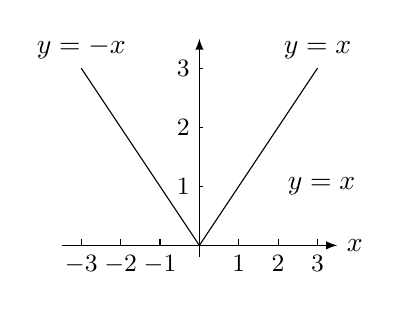
\begin{tikzpicture}[x=0.5cm,y=0.75cm]
\draw[-latex](-3.5,0)--(3.5,0)node[right]{$x$};
\draw[-latex](0,-0.2)--(0,3.5);
\foreach \x in {-3,-2,-1,1,2,3}{\draw(\x,0)node[below,font=\small]{$\x$}--++(0,0.1);}
\foreach \y in {1,2,3}{\draw(0,\y)node[left,font=\small]{$\y$}--++(0.1,0);}
\draw(-3,3)--(0,0)node[pos=0,above]{$y=-x$}--(3,3)node[pos=1,above]{$y=x$};
\draw(2,1)node[right]{$y=\abs{x}$};
\end{tikzpicture}
\caption{تفاعل کا کونا اس کو استمراری ہونے سے نہیں روکتا ہے (مثال \حوالہ{مثال_حد_استمراری_تفاعل_الف})۔}
\label{شکل_مثال_حد_استمراری_تفاعل_الف}
\end{minipage}\hfill
\begin{minipage}{0.45\textwidth}
\centering
\begin{tikzpicture}
\draw(0,0)--(6,0);
\draw[-latex](0.25,0)node[below]{$c$}node[circ]{}to[out=30,in=150]node[pos=0.5,sloped,fill=white,font=\small]{\RL{$c$ پر استمراری $f$}}(2.5,0)node[circ]{}node[below]{$f(c)$};
\draw[-latex] (2.5,0)to[out=30,in=150]node[pos=0.45,sloped,fill=white,font=\small]{\RL{$f(c)$ پر استمراری $g$}} (5.5,0)node[circ]{}node[below]{$g(f(c))$};
\draw[-latex](0.25,0) to [out=45,in=135]node[pos=0.5,sloped,above,font=\small]{\RL{$c$ پر استمراری $g\circ f$}} (5.5,0);
\end{tikzpicture}
\caption{مرکب تفاعل کی استمرار۔}
\label{شکل_مثال_حد_استمراری_تفاعل_ب}
\end{minipage}%
\end{figure}
\انتہا{مثال}
%=============================
\ابتدا{مثال}\موٹا{تکونیاتی تفاعل کی استمرار}\\
اگلے باب میں دکھایا جائے گا کہ \عددی{x} کی ہر قیمت پر \عددی{\sin x} اور \عددی{\cos x} استمراری ہے لہٰذا درج ذیل حاصل تقسیم ان تمام نقطوں پر استمراری ہوں گے جہاں یہ معین ہوں۔
\begin{align*}
\tan x=\frac{\sin x}{\cos x},\quad \cot x&=\frac{\cos x}{\sin x},\\
\sec x=\frac{1}{\cos x},\quad \csc x&=\frac{1}{\sin x}
\end{align*} 
\انتہا{مثال}
%===========================
\ابتدا{مسئلہ}\شناخت{مسئلہ_حد_مرکب_تفاعل_استمرار}\موٹا{مرکبات کی استمرار}\\
اگر \عددی{c} پر \عددی{f} اور \عددی{f(c)} پر \عددی{g} استمراری ہوں تب \عددی{c} پر \عددی{g\circ f} استمراری ہو گا (شکل \حوالہ{شکل_مثال_حد_استمراری_تفاعل_ب})۔
\انتہا{مسئلہ}
%====================
مرکب کی استمرار کسی بھی متناہی تعداد کے تفاعل کے لئے درست ہے۔بس اتنا ضروری ہے کہ ہر تفاعل اس نقطے پر استمراری ہو جہاں اس کو لاگو کیا گیا ہو۔

\ابتدا{مثال}
درج ذیل تفاعل اپنے اپنے دائرہ کار کے ہر نقطے پر استمراری ہیں۔
\begin{align*}
\text{(ا)}\quad y&=\sqrt{x}&& \text{\RL{مسئلہ \حوالہ{مسئلہ_حد_میل_کی_استمرار} اور \حوالہ{مسئلہ_حد_کثیر_رکنی_ناطق_استمرار} (کثیر رکنی کی ناطق طاقت)}}\\
\text{(ب)}\quad y&=\sqrt{x^2-2x-5} &&\text{\RL{مسئلہ \حوالہ{مسئلہ_حد_کثیر_رکنی_ناطق_استمرار} اور مسئلہ \حوالہ{مسئلہ_حد_مرکب_تفاعل_استمرار} (کثیر رکنی کی طاقت یا جذر کے ساتھ مرکب)}}\\
\text{(ج)}\quad y&=\frac{x\cos(x^{2/3})}{1+x^4}&&\text{\RL{مسئلہ \حوالہ{مسئلہ_حد_میل_کی_استمرار}، \حوالہ{مسئلہ_حد_کثیر_رکنی_ناطق_استمرار} اور \حوالہ{مسئلہ_حد_مرکب_تفاعل_استمرار} (طاقت، مرکب، حاصل ضرب، کثیر رکنی)}}\\
\text{(د)}\quad y&=\abs{\frac{x-2}{x^2-2}}&& \text{\RL{مسئلہ \حوالہ{مسئلہ_حد_کثیر_رکنی_ناطق_استمرار} اور \حوالہ{مسئلہ_حد_مرکب_تفاعل_استمرار} (حتمی قیمت اور ناطق تفاعل کا مرکب)}}
\end{align*}
\انتہا{مثال}
%=============================

\جزوحصہء{نقطے تک استمراری توسیع}
ہم نے مثال \حوالہ{مثال_حد_اجزاء_منسوخ_الف} میں دیکھا کہ ناطق تفاعل کا اس نقطے پر بھی حد موجود ہو سکتا ہے جہاں ناطق تفاعل کا نسب نما صفر کے برابر ہو۔اگر \عددی{f(c)} غیر معین ہو لیکن \عددی{\lim_{x\to c}f(x)=L}موجود ہو تب ہم درج ذیل نیا تفاعل \عددی{F(x)}  متعارف کر سکتے ہیں۔
\begin{align*}
F(x)=
\begin{cases}
f(x)&\text{\RL{اگر $x$ تفاعل $f$ کے دائرہ کار میں پایا جاتا ہو}}\\
L& \text{\RL{اگر $\,\,x=c\,\,$ ہو}}
\end{cases}
\end{align*}
تفاعل \عددی{F} نقطہ \عددی{x=c} پر بھی استمراری ہو گا۔ اس کو \عددی{f} کی نقطہ \عددی{x=c} تک \اصطلاح{استمراری توسیع}\فرہنگ{استمراری توسیع}\حاشیہب{continuous extension}\فرہنگ{continuous extension} کہتے ہیں اور توسیع شدہ تفاعل کو \اصطلاح{وسیع تفاعل}\فرہنگ{وسیع تفاعل}\حاشیہب{extended function}\فرہنگ{extended function} کہتے ہیں۔ناطق تفاعل \عددی{f} کے استمراری توسیع کو عموماً  مشترک اجزاء کی اسقاط کے ذریعہ حاصل کیا جاتا ہے۔

\ابتدا{مثال}
دکھائیں کہ درج ذیل تفاعل کا \عددی{x=2} پر استمراری توسیع ممکن ہے۔
\begin{align*}
f(x)=\frac{x^2+x-6}{x^2-4}
\end{align*}
حل:\quad
اگرچہ \عددی{f(2)} غیر معین ہے، \عددی{x\ne 2} پر درج ذیل لکھا جا سکتا ہے۔
\begin{align*}
f(x)=\frac{x^2+x-6}{x^2-4}=\frac{(x-2)(x+3)}{(x-2)(x+2)}=\frac{x+3}{x+2}
\end{align*}
درج ذیل تفاعل \عددی{x\ne 2} پر \عددی{f} کے برابر ہے  اور \عددی{x=2} پر استمراری ہے جہاں اس کی قیمت \عددی{\tfrac{5}{4}} ہے۔
\begin{align*}
F(x)=\frac{x+3}{x+2}
\end{align*}
یوں \عددی{f} کی نقطہ \عددی{x=2} تک توسیع تفاعل \عددی{F(x)} ہے  اور اس نقطے پر تفاعل کا حد درج ذیل ہے۔
\begin{align*}
\lim_{x\to 2}\frac{x^2+x-6}{x^2-4}=\lim_{x\to 2} f(x)=\frac{5}{4}
\end{align*}
تفاعل \عددی{f} کی ترسیم شکل \حوالہ{شکل_حد_استمراری_توسیع} میں دکھائی گئی ہے۔\عددی{F} کی بھی یہی ترسیم ہے مگر اس میں  \عددی{(2,\tfrac{5}{4})} پر سوراخ نہیں پایا جاتا ہے۔\عددی{f} اور \عددی{F} کا تعلق درج ذیل ہے۔
\begin{align*}
F=
\begin{cases}
f,&x\ne 2\\
\frac{5}{4},&x=2
\end{cases}
\end{align*}
%
\begin{figure}
\centering
\begin{subfigure}{0.5\textwidth}
\centering
\begin{tikzpicture}
\begin{axis}[small,axis lines=middle,xlabel={$x$},ylabel={$y$},ymin=-0.2,ymax=2.9,xmax=4.9,xmin=-1.5]
\addplot[domain=-1:4]{(x+3)/(x+2)};
\draw[dashed](axis cs:0,1.25)node[ocirc,solid]{}--(axis cs:2,1.25)node[ocirc,solid]{}--(axis cs:2,0)node[ocirc,solid]{};
\draw(axis cs:0,1.25)node[pin=170:{$\tfrac{5}{4}$}]{};
\draw(axis cs:2,2)node[]{$y=\frac{x^2+x-6}{x^2-4}$};
\end{axis}
\end{tikzpicture}
\caption{}
\end{subfigure}%
\begin{subfigure}{0.5\textwidth}
\centering
\begin{tikzpicture}
\begin{axis}[small,axis lines=middle,xlabel={$x$},ylabel={$y$},ymin=-0.2,ymax=2.9,xmax=4.9,xmin=-1.5]
\addplot[domain=-1:4]{(x+3)/(x+2)};
\draw[dashed](axis cs:0,1.25)--(axis cs:2,1.25)--(axis cs:2,0);
\draw(axis cs:0,1.25)node[pin=170:{$\tfrac{5}{4}$}]{};
\draw(axis cs:2,2)node[]{$y=\frac{x+3}{x+2}$};
\end{axis}
\end{tikzpicture}
\caption{}
\end{subfigure}%
\caption{تفاعل \عددی{f(x)} اور اس کی استمراری توسیع \عددی{F(x)}}
\label{شکل_حد_استمراری_توسیع}
\end{figure}
\انتہا{مثال}
%=========================

\جزوحصہء{وقفوں پر استمرار}
ایک تفاعل  اس صورت استمراری کہلاتا ہے جب یہ اپنے پورے دائرہ کار میں استمراری ہو۔ایسا تفاعل جو اپنے پورے دائرہ کار میں استمراری نہ ہو، دائرہ کار کے اندر مخصوص وقفوں میں استمراری ہو سکتا ہے۔
 
اگر \عددی{f} کے دائرہ کار کے اندر  وقفہ \عددی{I} میں  ہر اندرونی نقطہ \عددی{c} پر \عددی{\lim_{x\to c}f(x)=f(c)} ہو اور ہر آخری سر نقطہ جو \عددی{I} میں پایا جاتا ہو پر مناسب یک طرفہ حد اور تفاعل کی قیمت برابر ہوں تب \عددی{f}  \اصطلاح{وقفہ پر استمراری}\فرہنگ{استمراری!وقفہ پر}\حاشیہب{continuous on interval}\فرہنگ{continuous!on interval} کہلائے گا ۔جو تفاعل \عددی{I} پر استمراری ہو یہ تفاعل \عددی{I} کے اندر ہر وقفے پر استمراری ہو گا۔کثیر رکنی اور ناطق تفاعل ہر اس وقفے پر استمراری ہوں گے جن پر یہ معین ہوں۔


\ابتدا{مثال}\شناخت{مثال_حد_استمراری_تفاعل_مثالیں}\ترچھا{وقفوں پر استمراری تفاعل}\\
شکل \حوالہ{شکل_مثال_حد_استمراری_تفاعل_مثالیں} میں وقفوں پر  استمراری تفاعل کی مثالیں ترسیم کی گئی ہیں۔ 
\begin{figure}
\centering
\begin{subfigure}{0.5\textwidth}
\centering
\begin{tikzpicture}
\begin{axis}[axis equal,small,axis lines=middle,xlabel={$x$},ylabel={$y$},xmin=-2.25,xmax=2.75,ymax=2.75,xtick={\empty},ytick={2},ylabel style={at={(current axis.above origin)},anchor=south}]
\addplot[domain=0:180]({2*cos(x)},{2*sin(x)})node[pos=0.5,above right]{$y=\sqrt{4-x^2}$};
\draw(axis cs:-2,0)node[below]{$2$} (axis cs:2,0)node[below]{$2$};
\end{axis}
\end{tikzpicture}
\caption{\عددی{[-2,2]} پر استمراری}
\end{subfigure}%
\begin{subfigure}{0.5\textwidth}
\centering
\begin{tikzpicture}
\begin{axis}[axis equal,small,axis lines=middle,xlabel={$x$},ylabel={$y$},xtick={\empty},ytick={\empty},ylabel style={at={(current axis.above origin)},anchor=south},xlabel style={at={(current axis.right of origin)},anchor=west}]
\addplot[domain=0.25:4]{1/x}node[pos=0.25,right]{$y=\tfrac{1}{x}$};
\addplot[domain=-0.25:-4]{1/x};
\end{axis}
\end{tikzpicture}
\caption{\عددی{(-\infty,0)} اور \عددی{(0,\infty)} پر استمراری}
\end{subfigure}
\begin{subfigure}{0.5\textwidth}
\centering
\begin{tikzpicture}
\begin{axis}[small,axis lines=middle,xlabel={$x$},ylabel={$y$},xtick={\empty},ytick={\empty},ylabel style={at={(current axis.above origin)},anchor=south},xlabel style={at={(current axis.right of origin)},anchor=west},ymax=1.5,ymin=-0.2]
\addplot[thick] plot coordinates {(-4,0) (0,0) (0,1) (4,1)};
\draw(axis cs:0,0)node[ocirc]{}node[below left]{$0$} (axis cs:0,1)node[circ]{}node[left]{$1$};
\draw(axis cs:1,1)node[above right]{$y=U(x)$};
\end{axis}
\end{tikzpicture}
\caption{
\عددی{(-\infty,0)} اور \عددی{[0,\infty)} پر استمراری
}
\end{subfigure}%
\begin{subfigure}{0.5\textwidth}
\centering
\begin{tikzpicture}
\begin{axis}[small,axis lines=middle,xlabel={$x$},ylabel={$y$},xtick={\empty},ytick={-1,1},ylabel style={at={(current axis.above origin)},anchor=south},xlabel style={at={(current axis.right of origin)},anchor=west},ymax=1.5]
\addplot[domain=-200:200,samples=200]{cos(x)};
\draw(axis cs:90,1)node[right]{$y=\cos x$};
\end{axis}
\end{tikzpicture}
\caption{
\عددی{(-\infty,\infty)}  پر استمراری
}
\end{subfigure}%
\caption{وقفوں پر استمراری تفاعل (مثال \حوالہ{مثال_حد_استمراری_تفاعل_مثالیں})}
\label{شکل_مثال_حد_استمراری_تفاعل_مثالیں}
\end{figure}
\انتہا{مثال}
%=======================

وقفوں پر استمراری تفاعل ایسے خواص رکھتے ہیں جن کی بنا یہ  ریاضیات کے لئے نہایت اہم ثابت ہوتے ہیں۔ان میں ایک \اصطلاح{متوسط قیمت خاصیت}\فرہنگ{خاصیت!متوسط قیمت}\حاشیہب{intermediate value property}\فرہنگ{property!intermediate value} ہے۔ اگر دو اعداد کے بیچ تمام قیمتیں لئے بغیر تفاعل ان قیمتوں کو نہ لیتا ہو تب یہ تفاعل \اصطلاح{متوسط قیمت خاصیت} رکھتا ہے۔ 


\ابتدا{مسئلہ}\شناخت{مسئلہ_حد_متوسط_قیمت}\موٹا{مسئلہ متوسط قیمت}\\
فرض کریں کہ تفاعل \عددی{f} وقفہ \عددی{I} پر استمراری ہے جبکہ \عددی{a} اور \عددی{b} اس وقفے پر کوئی دو نقطے ہیں۔ تب اگر \عددی{f(a)} اور \عددی{f(b)} کے بیچ \عددی{y_0} ایک عدد ہو تب \عددی{a} اور \عددی{b} کے بیچ ایک ایسا عدد \عددی{c} پایا جائے گا کہ \عددی{f(c)=y_0} ہو (شکل \حوالہ{شکل_حد_بیچ_ہر_قیمت})۔
\begin{figure}
\centering
\begin{minipage}{0.45\textwidth}
\centering
\begin{tikzpicture}
\draw[-latex](-0.25,0)--(4.5,0)node[right]{$x$};
\draw[-latex](0,-0.2)--(0,2.5)node[above]{$y$};
\draw(0.5,0.5)coordinate(kA) to [out=-20,in=-135] (2,1.25)coordinate(kC) to [out=45,in=135] (4,2.25)coordinate(kB);
\draw[dashed] (kA)--($(0,0)!(kA)!(0,2.5)$)node[left]{$f(a)$};
\draw[dashed] (kA)--($(0,0)!(kA)!(4,0)$)node[below]{$a$};
\draw[dashed] (kB)--($(0,0)!(kB)!(0,2.5)$)node[left]{$f(b)$};
\draw[dashed] (kB)--($(0,0)!(kB)!(4,0)$)node[below]{$b$};
\draw[dashed] (kC)--($(0,0)!(kC)!(0,2.5)$)node[left]{$y_0$};
\draw[dashed] (kC)--($(0,0)!(kC)!(4,0)$)node[below]{$c$};
\draw(4,2.4)node[above]{$y=f(x)$};
\end{tikzpicture}
\caption{
وقفہ \عددی{[a,b]} پر استمراری تفاعل \عددی{f(a)} اور \عددی{f(b)} کے بیچ ہر قیمت رکھتا ہے 
}
\label{شکل_حد_بیچ_ہر_قیمت}
\end{minipage}\hfill
\begin{minipage}{0.45\textwidth}
\centering
\begin{tikzpicture}
\draw[-latex](-0.25,0)--(3,0)node[right]{$x$};
\draw[-latex](0,-0.2)--(0,2)node[above]{$y$};
\draw[thick](0,0)node[circ]{}node[below left]{$0$}--(1,0)node[ocirc]{}node[below]{$1$};
\draw(0,1)node[left]{$1$}--++(0.1,0);
\draw(1,1)node[circ]{};
\draw(2,1)node[above right]{$\begin{aligned} y&=\lfloor x \rfloor,\\ 0&\le x \le 1 \end{aligned}$};
\end{tikzpicture}
\caption{
تفاعل \عددی{y=\lfloor x\rfloor, 0\le x\le 1} کوئی بھی قیمت \عددی{f(0)=0} اور \عددی{f(1)=1} کے بیچ قبول نہیں کرتا ہے۔
}
\label{شکل_حد_بیچ_نہیں}
\end{minipage}%
\end{figure}  
\انتہا{مسئلہ}
%========================

متوسط قیمت مسئلے کا ثبوت، جو اعلٰی درجے کی کتابوں میں پایا جاتا ہے، حقیقی اعدادی نظام کی مکملیت پر منحصر ہے۔

اس مسئلے میں وقفہ \عددی{I} پر تفاعل \عددی{f} کی استمرار ضروری ہے۔اگر \عددی{I} میں صرف ایک نقطے پر بھی \عددی{f} غیر استمراری ہو تب یہ مسئلہ قابل استعمال نہیں ہو گا۔اس کی ایک مثال شکل \حوالہ{شکل_حد_بیچ_نہیں} میں دی گئی ہے۔


مسئلہ \حوالہ{مسئلہ_حد_متوسط_قیمت} کی بنا وقفہ \عددی{I} پر استمراری تفاعل کی ترسیم مسلسل ہوتی ہے، یعنی اس میں کوئی سوراخ یا خالی جگہ نہیں پائی جاتی ہے۔اس میں عددی صحیح زمین تفاعل \عددی{\lfloor x \rfloor} کی طرح چھلانگ  نہیں پائے جاتے ہیں اور نا ہی اس میں تفاعل \عددی{\tfrac{1}{x}} کی طرح علیحدہ علیحدہ شاخیں پائی جاتی ہیں۔

\جزوحصہء{تلاش جذر}
مساوات \عددی{f(x)=0} کے حل کو \عددی{f(x)} کا \اصطلاح{صفر}\فرہنگ{صفر}\حاشیہب{zero}\فرہنگ{zero} یا \اصطلاح{جذر}\فرہنگ{جذر}\حاشیہب{root}\فرہنگ{root} کہتے ہیں۔مسئلہ \حوالہ{مسئلہ_حد_متوسط_قیمت} کے تحت استمراری تفاعل کی صورت میں جس وقفے میں تفاعل کی علامت \عددی{(\pm)} تبدیل ہوتی ہو اس وقفے میں تفاعل کا صفر پایا جائے گا۔

اس حقیقت کو استعمال کرتے ہوئے ہم  \عددی{f(x)=0} طرز کی مساوات کا حل بذریعہ کمپیوٹر تلاش کر سکتے ہیں  (جہاں \عددی{f} استمراری ہے)۔ مساوات کی ترسیم \عددی{x} محور کو \عددی{f} کی جذر پر قطع کرتی ہے۔ہم \عددی{y=f(x)} کو کسی بڑے وقفے پر ترسیم کرتے ہوئے دیکھتے ہیں کہ یہ کہاں \عددی{x} محور کو قطع کرتی ہے۔ہم ان نقطوں  کو باری باری قریب سے دیکھ کر جذر کی اندازاً قیمت دیکھتے ہیں۔اب ہم جذر کی اس اندازاً  قیمت کے گرد چھوٹے وقفے پر مساوات ترسیم کرتے ہوئے جذر کی مزید بہتر قیمت تلاش کرتے ہیں۔اس عمل کو جتنی مرتبہ ضرورت ہو دہراتے ہوئے درکار درستگی تک کا جذر تلاش کیا جا سکتا ہے۔شکل \حوالہ{شکل_حد_جذر_بذریعہ_ترسیم} میں، قدم با قدم، اس عمل سے  \عددی{x^3-0.25x^2-1.25x-0.75=0} کا  جذر حاصل کرنا دکھایا گیا ہے۔

ترسیم سے مساوات کو حل کرتے ہوئے تفاعل کے جذر حاصل کرنے میں زیادہ وقت درکار ہوتا ہے۔اس سے کم دورانیے میں جذر کو بذریعہ اعدادی تراکیب حاصل کیا جا سکتا ہے جن پر بعد میں غور کیا جائے گا۔
\begin{figure}
\centering
\begin{subfigure}{0.3\textwidth}
\centering
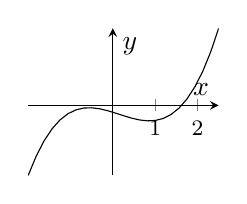
\begin{tikzpicture}
\begin{axis}[small,axis lines=middle,xtick={1,2},ytick={\empty},xlabel={$x$},ylabel={$y$},width=4cm]
\addplot[domain=-2:2.5]{-0.75+x*(x-1.45)*(x+1)};
\end{axis}
\end{tikzpicture}
\caption{جذر  (صفر) \عددی{1} اور \عددی{2} کے بیچ پایا جاتا ہے۔}
\end{subfigure}\hfill
\begin{subfigure}{0.3\textwidth}
\centering
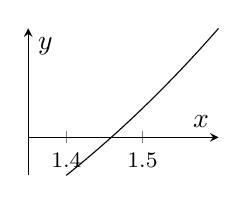
\begin{tikzpicture}
\begin{axis}[small,axis lines=middle,ytick={\empty},xlabel={$x$},ylabel={$y$},width=4cm,xmin=1.35,xtick={1.4,1.5}]
\addplot[domain=1.4:1.6]{-0.75+x*(x-1.25)*(x+1)};
\end{axis}
\end{tikzpicture}
\caption{جذر (صفر) \عددی{1.4} اور \عددی{1.5} کے بیچ پایا جاتا ہے۔}
\end{subfigure}\hfill
\begin{subfigure}{0.3\textwidth}
\centering
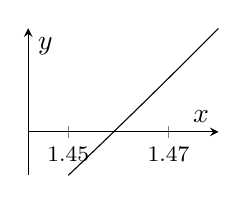
\begin{tikzpicture}
\begin{axis}[small,axis lines=middle,ytick={\empty},xlabel={$x$},ylabel={$y$},width=4cm,xmin=1.442,xtick={1.45,1.47}]
\addplot[domain=1.45:1.48]{-0.75+x*(x-1.25)*(x+1)};
\end{axis}
\end{tikzpicture}
\caption{جذر (صفر) \عددی{1.45} اور \عددی{1.47} کے بیچ پایا جاتا ہے۔}
\end{subfigure}
\begin{subfigure}{0.3\textwidth}
\centering
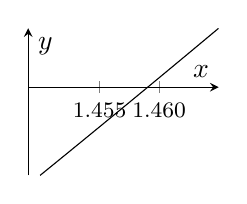
\begin{tikzpicture}
\begin{axis}[small,axis lines=middle,ytick={\empty},xlabel={$x$},ylabel={$y$},width=4cm,xtick={1.455,1.460},xticklabels={$1.455$,$1.460$},xmin=1.449]
\addplot[domain=1.45:1.465]{-0.75+x*(x-1.25)*(x+1)};
\end{axis}
\end{tikzpicture}
\caption{جذر (صفر) \عددی{1.455} اور \عددی{1.460} کے بیچ پایا جاتا ہے۔}
\end{subfigure}\hfill
\begin{subfigure}{0.3\textwidth}
\centering
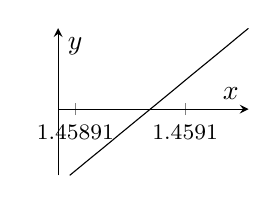
\begin{tikzpicture}
\begin{axis}[small,axis lines=middle,ytick={\empty},xlabel={$x$},ylabel={$y$},width=4cm,xtick={1.45891,1.4591},xticklabels={$1.45891$,$1.4591$},xmin=1.45888]
\addplot[domain=1.4589:1.4592]{-0.75+x*(x-1.25)*(x+1)};
\end{axis}
\end{tikzpicture}
\caption{جذر (صفر) \عددی{1.45891} اور \عددی{1.4591} کے بیچ پایا جاتا ہے۔}
\end{subfigure}\hfill
\begin{subfigure}{0.3\textwidth}
\centering
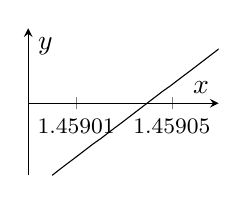
\begin{tikzpicture}
\begin{axis}[small,axis lines=middle,ytick={\empty},xlabel={$x$},ylabel={$y$},width=4cm,xtick={1.45901,1.45905},xticklabels={$1.45901$,$1.45905$},xmin=1.45899]
\addplot[domain=1.4590:1.45907]{-0.75+x*(x-1.25)*(x+1)};
\end{axis}
\end{tikzpicture}
\caption{جذر (صفر) \عددی{1.45901} اور \عددی{1.45905} کے بیچ پایا جاتا ہے۔}
\end{subfigure}
\caption{
ترسیم کے ذریعہ  \عددی{x^3-0.25x^2-1.25x-0.75=0} کے جذر کا قدم با قدم  حصول۔
}
\label{شکل_حد_جذر_بذریعہ_ترسیم}
\end{figure}


\حصہء{سوالات}
\موٹا{استمرار بذریعہ ترسیم}\\
سوال \حوالہ{سوال_حد_ترسیم_استمرار_الف} تا سوال \حوالہ{سوال_حد_ترسیم_استمرار_د} میں دریافت کریں کہ آیا تفاعل وقفہ \عددی{[-1,3]} پر استمراری ہے۔نا ہونے کی صورت میں کہاں تفاعل غیر استمراری ہے اور ایسا کیوں ہے؟

\ابتدا{سوال}\شناخت{سوال_حد_ترسیم_استمرار_الف}
تفاعل \عددی{y=f(x)} جسے شکل \حوالہ{شکل_سوال_حد_ترسیم_استمرار_الف}-ا میں دکھایا گیا ہے۔
\begin{figure}
\centering
\begin{subfigure}{0.25\textwidth}
\centering
\begin{tikzpicture}[x=0.5cm]
\draw[-latex](-1.25,0)--(3.5,0)node[right]{$x$};
\draw[-latex](0,-0.2)--(0,2.5)node[above]{$y$};
\foreach \x in {-1,1,2,3}{\draw(\x,0)node[below]{$\x$}--++(0,0.1);}
\foreach \y in {1,2}{\draw(0,\y)node[left]{$\y$}--++(0.1,0);}
\draw(-1,0.25)node[circ]{} to [out=45,in=150](2,1)node[ocirc]{}to[out=-30,in=-110](3,2)node[circ]{};
\draw(1,2.5)node[right]{$y=f(x)$};
\end{tikzpicture}
\caption{}
\end{subfigure}%
\begin{subfigure}{0.25\textwidth}
\centering
\begin{tikzpicture}[x=0.5cm]
\draw[-latex](-1.25,0)--(3.5,0)node[right]{$x$};
\draw[-latex](0,-0.2)--(0,2.5)node[above]{$y$};
\foreach \x in {-1,1,2,3}{\draw(\x,0)node[below]{$\x$}--++(0,0.1);}
\foreach \y in {1,2}{\draw(0,\y)node[left]{$\y$}--++(0.1,0);}
\draw(-1,0.25)node[circ]{} to [out=45,in=-110](2,2)to[out=-60,in=170](3,1)node[ocirc]{}(3,1.5)node[circ]{};
\draw(1,2.5)node[right]{$y=g(x)$};
\end{tikzpicture}
\caption{}
\end{subfigure}%
\begin{subfigure}{0.25\textwidth}
\centering
\begin{tikzpicture}[x=0.5cm]
\draw[-latex](-1.25,0)--(3.5,0)node[right]{$x$};
\draw[-latex](0,-0.2)--(0,2.5)node[above]{$y$};
\foreach \x in {-1,1,2,3}{\draw(\x,0)node[below]{$\x$}--++(0,0.1);}
\foreach \y in {1,2}{\draw(0,\y)node[left]{$\y$}--++(0.1,0);}
\draw(-1,2)node[circ]{}--(1,1)--(2,2)--(3,2)node[circ]{};
\draw(1,2.5)node[right]{$y=h(x)$};
\end{tikzpicture}
\caption{}
\end{subfigure}%
\begin{subfigure}{0.25\textwidth}
\centering
\begin{tikzpicture}[x=0.5cm]
\draw[-latex](-1.25,0)--(3.5,0)node[right]{$x$};
\draw[-latex](0,-0.2)--(0,2.5)node[above]{$y$};
\foreach \x in {-1,1,2,3}{\draw(\x,0)node[below]{$\x$}--++(0,0.1);}
\foreach \y in {1,2}{\draw(0,\y)node[left]{$\y$}--++(0.1,0);}
\draw(-1,0)node[circ]{}--(1,1.5)node[ocirc]{} (1,0)node[circ]{}--(3,2)node[circ]{};
\draw(1,2.5)node[right]{$y=k(x)$};
\end{tikzpicture}
\caption{}
\end{subfigure}%
\caption{اشکال برائے سوال \حوالہ{سوال_حد_ترسیم_استمرار_الف} تا سوال \حوالہ{سوال_حد_ترسیم_استمرار_د}}
\label{شکل_سوال_حد_ترسیم_استمرار_الف}
\end{figure}
\انتہا{سوال}
%=======================
\ابتدا{سوال}
تفاعل \عددی{y=g(x)} جسے شکل \حوالہ{شکل_سوال_حد_ترسیم_استمرار_الف}-ب میں دکھایا گیا ہے۔
\انتہا{سوال}
%=========================
\ابتدا{سوال}
تفاعل \عددی{y=h(x)} جسے شکل \حوالہ{شکل_سوال_حد_ترسیم_استمرار_الف}-ج میں دکھایا گیا ہے۔
\انتہا{سوال}
%=========================
\ابتدا{سوال}\شناخت{سوال_حد_ترسیم_استمرار_د}
تفاعل \عددی{y=k(x)} جسے شکل \حوالہ{شکل_سوال_حد_ترسیم_استمرار_الف}-د میں دکھایا گیا ہے۔
\انتہا{سوال}
%=========================
سوال \حوالہ{سوال_حد_تفاعل_ایک_الف} تا سوال \حوالہ{سوال_حد_تفاعل_ایک_ب} درج ذیل تفاعل کے بارے میں ہیں جس کو شکل \حوالہ{شکل_سوال_حد_تفاعل_ایک_الف} میں ترسیم کیا گیا ہے
\begin{align*}
f(x)=
\begin{cases}
x^2-1,&-1\le x <0\\
2x,&0<x<1\\
1,&x=1\\
-2x+4,&1<x<2\\
0,&2<x<3
\end{cases}
\end{align*}
%
\begin{figure}
\centering
\begin{tikzpicture}
\draw[-latex](-1.5,0)--(3.5,0)node[right]{$x$};
\draw[-latex](0,-1.5)--(0,2.5)node[above]{$y$};
\foreach \x in {-1,1,2,3}{\draw(\x,0)node[below]{$\x$}--++(0,0.1);}
\foreach \y in {-1,1,2}{\draw(0,\y)node[left]{$\y$}--++(0.1,0);}
\draw[thick,domain=-1:0] plot ({\x},{\x*\x-1});
\draw(-0.75,-0.75)node[left]{$y=x^2-1$} (-1,0)node[circ]{}(0,-1)node[ocirc]{};
\draw[thick](0,0)node[ocirc]{}--(1,2)node[pos=0.5,fill=white,left,xshift={-2mm}]{$y=2x$}node[ocirc]{}node[right]{$(1,2)$}--(2,0)node[pos=0.5,right]{$y=-2x+4$}node[ocirc]{}--(3,0)node[ocirc]{} (1,1)node[circ]{}node[below]{$(1,1)$};
\draw(3,2)node[]{$y=f(x)$};
\end{tikzpicture}
\caption{ترسیم برائے سوال \حوالہ{سوال_حد_تفاعل_ایک_الف} تا سوال \حوالہ{سوال_حد_تفاعل_ایک_ب}}
\label{شکل_سوال_حد_تفاعل_ایک_الف}
\end{figure}
\ابتدا{سوال}\شناخت{سوال_حد_تفاعل_ایک_الف}
(ا) \quad کیا \عددی{f(-1)} موجود ہے؟\\
(ب)  \quad کیا \عددی{\lim_{x\to -1^+}f(x)} موجود ہے؟\\
(ج) \quad کیا \عددی{\lim_{x\to -1^+}f(x)=f(-1)} ہے؟\\
(د) \quad کیا \عددی{x=-1} پر \عددی{f(x)} استمراری ہے؟
\انتہا{سوال}
%====================
\ابتدا{سوال}
(ا) \quad کیا \عددی{f(x)} موجود ہے؟\\
(ب) \quad  کیا \عددی{\lim_{x\to 1}f(x)} موجود ہے؟\\
(ج) \quad  کیا \عددی{\lim_{x\to 1}f(x)=f(1)} ہے؟\\
(د)  \quad  کیا \عددی{x=1} پر \عددی{f} استمراری ہے؟
\انتہا{سوال}
%=======================
\ابتدا{سوال}
(ا) \quad کیا \عددی{x=2} پر \عددی{f} معین ہے؟\\
(ب) \quad  کیا \عددی{ش=2} پر \عددی{f} استمراری ہے؟ 
\انتہا{سوال}
%=======================
\ابتدا{سوال}
\عددی{x} کی کس قیمت پر \عددی{f} استمراری ہے؟
\انتہا{سوال}
%========================
\ابتدا{سوال}
\عددی{x=2} پر توسیع کردہ تفاعل کو استمراری بنانے کی خاطر \عددی{f(2)} کی کیا قیمت ہونی چاہیے؟
\انتہا{سوال}
%=======================
\ابتدا{سوال}\شناخت{سوال_حد_تفاعل_ایک_ب}
\عددی{f(1)} کی کیا قیمت غیر استمرار کو ختم کرے گی؟
\انتہا{سوال}
%=======================
\موٹا{پرکھ استمرار کا استعمال}\\
کن نقطوں پر سوال \حوالہ{سوال_حد_کیا_ممکن_الف} اور سوال \حوالہ{سوال_حد_کیا_ممکن_ب} میں دیے گئے تفاعل غیر استمراری ہیں۔ کن نقطوں پر غیر استمرار ختم کیا جا سکتا ہے؟ کن نقطوں پر غیر استمرار ختم نہیں کیا جا سکتا ہے؟ اپنے جوابات کی وجہ پیش کریں۔ 

\ابتدا{سوال}\شناخت{سوال_حد_کیا_ممکن_الف}
حصہ \حوالہ{حصہ_حد_توسیع_حد} میں سوال \حوالہ{سوال_حد_فقرے_درست_الف} کے تفاعل۔
\انتہا{سوال}
%=======================
\ابتدا{سوال}\شناخت{سوال_حد_کیا_ممکن_ب}
حصہ \حوالہ{حصہ_حد_توسیع_حد} سوال \حوالہ{سوال_حد_فقرے_درست_ب} میں کے تفاعل۔
\انتہا{سوال}
%=======================
سوال \حوالہ{سوال_حد_کیا_استمراری_ہیں_الف} تا سوال \حوالہ{سوال_حد_کیا_استمراری_ہیں_ب}  میں کن نقطوں پر تفاعل استمراری ہیں۔

\ابتدا{سوال}\شناخت{سوال_حد_کیا_استمراری_ہیں_الف}
$y=\tfrac{1}{x-2}-3x$
\انتہا{سوال}
%==========================
\ابتدا{سوال}
$y=\tfrac{1}{(x+2)^2}+4$
\انتہا{سوال}
%======================
\ابتدا{سوال}
$y=\tfrac{x+1}{x^2-4x+3}$
\انتہا{سوال}
%======================
\ابتدا{سوال}
$y=\tfrac{x+3}{x^2-3x-10}$
\انتہا{سوال}
%======================
\ابتدا{سوال}
$y=\abs{x-1}+\sin x$
\انتہا{سوال}
%======================
\ابتدا{سوال}
$y=\tfrac{1}{\abs{x}+1}-\tfrac{x^2}{2}$
\انتہا{سوال}
%======================
\ابتدا{سوال}
$y=\tfrac{\cos x}{x}$
\انتہا{سوال}
%======================
\ابتدا{سوال}
$y=\tfrac{x+2}{\cos x}$
\انتہا{سوال}
%======================
\ابتدا{سوال}
$y=\csc x$
\انتہا{سوال}
%======================
\ابتدا{سوال}
$y=\tan \tfrac{\pi x}{2}$
\انتہا{سوال}
%======================
\ابتدا{سوال}
$y=\tfrac{x\tan x}{x^2+1}$
\انتہا{سوال}
%======================
\ابتدا{سوال}
$y=\tfrac{\sqrt{x^4+1}}{1+\sin^2x}$
\انتہا{سوال}
%======================
\ابتدا{سوال}
$y=\sqrt{2x+3}$
\انتہا{سوال}
%======================
\ابتدا{سوال}
$y=\sqrt[\leftroot{-2}4]{3x-1}$
\انتہا{سوال}
%======================
\ابتدا{سوال}
$y=(2x-1)^{1/3}$
\انتہا{سوال}
%======================
\ابتدا{سوال}\شناخت{سوال_حد_کیا_استمراری_ہیں_ب}
$y=(2-x)^{1/5}$
\انتہا{سوال}
%======================

\موٹا{مرکب تفاعل کے حد}\\
سوال \حوالہ{سوال_حد_مرکب_تفاعل_الف} تا سوال \حوالہ{سوال_حد_مرکب_تفاعل_ب} میں حد تلاش کریں۔

\ابتدا{سوال}\شناخت{سوال_حد_مرکب_تفاعل_الف}
$\lim\limits_{x\to \pi} \sin(x-\sin x)$
\انتہا{سوال}
%======================
\ابتدا{سوال}
$\lim\limits_{t\to 0} \sin(\tfrac{\pi}{2}\cos (\tan t))$
\انتہا{سوال}
%======================
\ابتدا{سوال}
$\lim\limits_{y\to 1} \sec(y\sec^2 y-\tan^2 y-1)$
\انتہا{سوال}
%======================
\ابتدا{سوال}
$\lim\limits_{x\to 0} \tan(\tfrac{\pi}{4}\cos(\sin x^{1/3}))$
\انتہا{سوال}
%======================
\ابتدا{سوال}
$\lim\limits_{t\to 0} \cos(\tfrac{\pi}{\sqrt{19-3\sec 2t}})$
\انتہا{سوال}
%======================
\ابتدا{سوال}\شناخت{سوال_حد_مرکب_تفاعل_ب}
$\lim\limits_{x\to \pi/6} \sqrt{\csc^2 x+5\sqrt{3}\tan x}$
\انتہا{سوال}
%======================
\موٹا{استمراری توسیع}

\ابتدا{سوال}
\عددی{g(3)} کی تعریف یوں کریں کہ \عددی{x=3} پر \عددی{g(x)=\tfrac{x^2-9}{x-3}} کی  استمراری توسیع  ہو۔
\انتہا{سوال}
%=======================
\ابتدا{سوال}
\عددی{h(2)} کی تعریف یوں کریں کہ \عددی{t=2} پر \عددی{h(t)=\tfrac{t^2+3t-10}{t-2}} کی  استمراری توسیع  ہو۔
\انتہا{سوال}
%=======================
\ابتدا{سوال}
\عددی{f(1)} کی تعریف یوں کریں کہ \عددی{s=1} پر \عددی{f(s)=\tfrac{s^3-1}{s^2-1}} کی  استمراری توسیع  ہو۔
\انتہا{سوال}
%=======================
\ابتدا{سوال}
\عددی{g(4)} کی تعریف یوں کریں کہ \عددی{x=4} پر \عددی{g(x)=\tfrac{x^2-16}{x^2-3x-4}} کی  استمراری توسیع  ہو۔
\انتہا{سوال}
%=======================
\ابتدا{سوال}
\عددی{a} کی کس قیمت کے لئے ہر \عددی{x} پر 
$\,\,f(x)=\begin{cases} x^2-1,&x<3\\ 2ax,&x\ge 3  \end{cases}\,\,$
استمراری ہے؟
\انتہا{سوال}
%==============
\ابتدا{سوال}
\عددی{b} کی کس قیمت کے لئے ہر \عددی{x} پر 
$\,\,g(x)=\begin{cases} x,&x<-2\\ bx^2,&x\ge -2  \end{cases}\,\,$
استمراری ہے؟
\انتہا{سوال}
%==============

\موٹا{استمراری توسیع۔ کمپیوٹر کا استعمال}\\
سوال \حوالہ{سوال_حد_تلاش_توسیع_الف} تا سوال \حوالہ{سوال_حد_تلاش_توسیع_ب} میں تفاعل \عددی{f} کو ترسیم کرتے ہوئے دیکھیں کہ آیا  مبدا پر اس کا استمراری توسیع پایا جاتا ہے۔اگر ایسا ہو تب \عددی{x=0} پر وسیع تفاعل کی موزوں قیمت تلاش کریں۔ اگر تفاعل کی استمراری توسیع  ممکن نہ ہو، تب کیا اس کو مبدا پر دائیں یا بائیں سے استمراری بنایا جا سکتا ہے اور ایسی صورت میں مبدا پر وسیع تفاعل کی قیمت کیا ہو گی؟

\ابتدا{سوال}\شناخت{سوال_حد_تلاش_توسیع_الف}
$f(x)=\tfrac{10^x-1}{x}$
\انتہا{سوال}
%=======================
\ابتدا{سوال}
$f(x)=\tfrac{10^{\abs{x}}-1}{x}$
\انتہا{سوال}
%=======================
\ابتدا{سوال}
$f(x)=\tfrac{\sin x}{\abs{x}}$
\انتہا{سوال}
%=======================
\ابتدا{سوال}\شناخت{سوال_حد_تلاش_توسیع_ب}
$f(x)=(1+2x)^{1/x}$
\انتہا{سوال}
%=======================

\موٹا{نظریہ اور مثالیں}

\ابتدا{سوال}
ایک استمراری تفاعل  کی قیمت \عددی{x=0} پر منفی  اور \عددی{x=1} پر مثبت ہے۔\عددی{x=0} اور \عددی{x=1} کے بیچ مساوات \عددی{f(x)=0} کا کم سے کم ایک حل کیوں  پایا جائے گا؟ ایک خاکہ کھینچ کر وجہ بیان کریں۔
\انتہا{سوال}
%========================
\ابتدا{سوال}
مساوات \عددی{\cos x=x} کا کم سے کم ایک حل کیوں پایا جائے گا؟
\انتہا{سوال}
%===================
\ابتدا{سوال}
دکھائیں کہ وقفہ \عددی{[-4,4]} میں مساوات \عددی{x^3-15x+1=0} کے تین حل پائے جاتے ہیں۔
\انتہا{سوال}
%===================
\ابتدا{سوال}
دکھائیں کہ کسی \عددی{x} پر تفاعل \عددی{F(x)=(x-a)^2(x-b)^2+x} کی قیمت \عددی{\tfrac{a+b}{2}} ہو گی۔
\انتہا{سوال}
%=================
\ابتدا{سوال}
دکھائیں کہ \عددی{c} کی ایسی قیمتیں پائی جاتی ہیں جن پر تفاعل \عددی{f(x)=x^3-8x+10} کی قیمت (ا) \عددی{\pi}؛ (ب) \عددی{-\sqrt{3}}؛ (ج) \عددی{\num{5000000}} ہوں گی۔
\انتہا{سوال}
%=======================
\ابتدا{سوال}
سمجھائیں کہ درج ذیل جملے ایک ہی معلومات پوچھتی ہیں۔\\
(ا)\quad  \عددی{f(x)=x^3-3x-1} کے جذر تلاش کریں۔\\
(ب)\quad  اس نقطے کا \عددی{x} محدد تلاش کریں جہاں \عددی{y=x^3} اور \عددی{y=3x+1} ایک دوسرے کو قطع کرتی ہیں۔\\
(ج)\quad  وہ تمام قیمتیں تلاش کریں جن پر \عددی{x^3-3x=1} ہو گا۔\\
(د)\quad  ان نقطوں کے \عددی{x} محدد تلاش کریں جہاں منحنی \عددی{y=x^3-3x} خط \عددی{y=1} کو قطع کرتی ہے۔\\
(ہ)\quad  مساوات \عددی{x^3-3x-1=0} کو حل کریں۔
\انتہا{سوال}
%=========================
\ابتدا{سوال}
ایسا تفاعل \عددی{f(x)} کی مثال دیں جو تمام \عددی{x} پر استمراری ہو  ماسوائے \عددی{x=2} پر جہاں اس کا قابل ہٹاو عدم استمرار پایا جاتا ہے۔بتلائیں کہ آپ کیسے جانتے ہیں کہ \عددی{x=2} پر عدم استمرار پایا جاتا ہے اور کہ یہ عدم استمرار قابل ہٹاو ہے۔
\انتہا{سوال}
%=================
\ابتدا{سوال}
ایسا تفاعل \عددی{g(x)} کی مثال دیں جو تمام \عددی{x} پر استمراری ہو  ماسوائے \عددی{x=-1} پر جہاں اس کا نا قابل ہٹاو عدم استمرار پایا جاتا ہے۔بتلائیں کہ آپ کیسے جانتے ہیں کہ \عددی{x=1} پر عدم استمرار پایا جاتا ہے اور کہ یہ عدم استمرار نا قابل ہٹاو ہے۔
\انتہا{سوال}
%=================
\ابتدا{سوال}\ترچھا{تمام نقطوں پر غیر استمراری تفاعل}\\
(ا)\quad اس حقیقت کو برائے کار لاتے ہوئے، کہ حقیقی اعداد کا ہر غیر خالی وقفہ ناطق اور غیر ناطق اعداد پر مشتمل ہے، دکھائیں کہ درج ذیل تفاعل ہر نقطے پر عدم استمراری ہے۔
\begin{align*}
f(x)=
\begin{cases}
1& x\,\,\text{\RL{ناطق}}\\
0&x\,\,\text{\RL{غیر ناطق}}
\end{cases}
\end{align*}
(ب)\quad  کیا کسی نقطے پر \عددی{f} دائیں استمراری یا بائیں استمراری ہے؟
\انتہا{سوال}
%======================
\ابتدا{سوال}
اگر \عددی{0\le x\le 1} پر \عددی{f(x)} اور \عددی{g(x)} استمراری ہوں تب کیا \عددی{[0,1]} کے کسی نقطے پر \عددی{h(x)=f(x)\cdot g(x)} غیر استمراری ہو سکتا ہے؟ اپنے جواب کی وجہ پیش کریں۔
\انتہا{سوال}
%=======================
\ابتدا{سوال}
اگر تفاعل \عددی{h(x)=f(h)\cdot g(x)} نقطہ \عددی{x=0} پر استمراری ہو تب کیا \عددی{f(x)} اور \عددی{g(x)} ضرور \عددی{x=0} پر استمراری ہوں گے؟ اپنے جواب کی وجہ پیش کریں۔
\انتہا{سوال}
%=======================
\ابتدا{سوال}
ایسے تفاعل \عددی{f(x)} اور \عددی{g(x)} کی مثال دیں جو \عددی{x=0} پر استمراری ہوں لیکن ان کا مرکب تفاعل \عددی{f\circ g} نقطہ \عددی{x=0} پر عدم استمراری ہو۔ کیا یہ مسئلہ \حوالہ{مسئلہ_حد_مرکب_تفاعل_استمرار} کی خلاف ورزی کرتا ہے؟ اپنے جواب کی وجہ پیش کریں۔
\انتہا{سوال}
%=========================
\ابتدا{سوال}
کیا یہ کہنا درست ہو گا کہ جو تفاعل کسی وقفے پر کبھی صفر نہیں ہوتا ہے وہ تفاعل اس وقفہ پر کبھی علامت تبدیل نہیں کرتا ہے؟اپنے جواب کی وجہ پیش کریں۔
\انتہا{سوال}
%=======================
\ابتدا{سوال}
کیا یہ درست ہے کہ ربڑ کی پٹی کو دونوں سروں سے کھینچنے کے با وجود پٹی پر ایک نقطہ ایسا پایا جاتا ہے جو اپنی جگہ بر قرار رکھتا ہے؟ اپنے جواب کی وجہ پیش کریں۔
\انتہا{سوال}
%=========================
\ابتدا{سوال}\ترچھا{مسئلہ مقررہ نقطہ}\\
فرض کریں کہ وقفہ \عددی{0,1} میں تفاعل \عددی{f} استمراری ہے اور \عددی{[0,1]} میں ہر \عددی{x} کے لئے \عددی{0\le f(x)\le 1} ہے۔دکھائیں کہ \عددی{[0,1]} میں ایسا نقطہ \عددی{c} پایا جاتا ہے جس پر \عددی{f(c)=c} ہو گا۔ \عددی{c} کو \عددی{f} کا \اصطلاح{مقررہ نقطہ}\فرہنگ{مقررہ نقطہ}\حاشیہب{fixed point}\فرہنگ{fixed point} کہتے ہیں۔
\انتہا{سوال}
%=======================
\ابتدا{سوال}\ترچھا{استمراری تفاعل کی علامت بر قرار رکھنے کی خاصیت}\\
فرض کریں کہ وقفہ \عددی{(a,b)} پر تفاعل \عددی{f} معین ہے اور نقطہ \عددی{c} جہاں \عددی{f} استمراری ہے پر  \عددی{f(c)\ne 0} ہے۔ دکھائیں کے \عددی{c} کے ارد گرد وقفہ \عددی{c-\delta,c+\delta} میں \عددی{f} کی علامت وہی ہو گی جو \عددی{c} پر \عددی{f(c)} کی ہے۔ یہ ایک غیر معمولی نتیجہ ہے۔ اگرچہ \عددی{(a,b)} پر \عددی{f} معین ہے، کسی بھی نقطے پر تفاعل کا استمراری ہونا ضروری نہیں ہے ماسوائے نقطہ \عددی{c} پر۔ اس کے ساتھ شرط \عددی{f(c)\ne 0} ملانے سے \عددی{f} غیر صفر حاصل ہوتا ہے یعنی پورے وقفے پر \عددی{f} مثبت یا منفی ہو گا۔
\انتہا{سوال}
%========================
\ابتدا{سوال}
دکھائیں کہ حصہ \حوالہ{حصہ_حد_قواعد} میں مسئلہ \حوالہ{مسئلہ_حد_قواعد-الف} سے اس حصے کا مسئلہ \حوالہ{مسئلہ_حد_میل_کی_استمرار} کس طرح اخذ کیا جا سکتا ہے۔ 
\انتہا{سوال}
%=====================
\ابتدا{سوال}
دکھائیں کہ حصہ \حوالہ{حصہ_حد_قواعد} میں مسئلہ \حوالہ{مسئلہ_حد_قواعد_ب} اور مسئلہ \حوالہ{مسئلہ_حد_قواعد_پ} سے موجودہ حصے کا مسئلہ \حوالہ{مسئلہ_حد_کثیر_رکنی_ناطق_استمرار} کس طرح اخذ کیا جا سکتا ہے؟
\انتہا{سوال}
%=======================

\موٹا{سوال کا حل بذریعہ ترسیم}\\
کمپیوٹر کی مدد سے ترسیم کھینچ کر درج ذیل سوالات حل کریں۔

\ابتدا{سوال}
$x^3-3x-1=0$
\انتہا{سوال}
%============= 
\ابتدا{سوال}
$2x^3-2x^2-2x+1=0$
\انتہا{سوال}
%============= 
\ابتدا{سوال}
$x(x-1)^2=1$  
ایک جذر حاصل کریں۔
\انتہا{سوال}
%============= 
\ابتدا{سوال}
$x^x=2$
\انتہا{سوال}
%============= 
\ابتدا{سوال}
$\sqrt{x}+\sqrt{x+1}=4$
\انتہا{سوال}
%============= 
\ابتدا{سوال}
$x^3-15x+1=0$
تین جذر تلاش کریں۔
\انتہا{سوال}
%=============
\ابتدا{سوال}
$\cos x=x$
ایک جذر تلاش کریں اور ریڈیئن استعمال کرنا مت بھولیں۔
\انتہا{سوال}
%============= 
\ابتدا{سوال}
$2\sin x=x$
ایک جذر تلاش کریں اور ریڈیئن استعمال کرنا مت بھولیں۔
\انتہا{سوال}
%============= 


\حصہ{مماسی خط}
حصہ \حوالہ{حصہ_حد_تبدیلی_کی_شرح_اور_حد} میں سیکنٹ اور مماس پر بحث کی گئی۔اس بحث کو اس حصے میں جاری رکھتے ہیں۔ہم سیکنٹ کی ڈھلوان کا حد تلاش کرتے ہوئے منحنی کا مماس حاصل کریں گے۔

\جزوحصہء{منحنی کے مماس سے کیا مراد ہے؟} 
دائرے کی مماس  کا مطلب سیدھا سادہ ہے۔نقطہ \عددی{N} پر دائرہ \عددی{C} کے مماس سے مراد خط \عددی{L} ہے جو نقطہ \عددی{N} سے گزرتا ہے  اور  \عددی{N} پر رداس کو عمودی  ہے (شکل \حوالہ{شکل_حد_مماس_دائرہ})۔  نقطہ \عددی{N} پر کسی اور منحنی \عددی{C} کے مماس سے کیا مطلب ہے؟ دائرے کی جیومیٹری کو دیکھ کر ہم کہہ سکتے ہیں کہ مماس کا مطلب درج ذیل میں سے ایک ہو سکتا ہے۔
\begin{enumerate}[1.]
\item
\عددی{N} سے \عددی{C} کی مرکز تک خط کو عمودی خط \عددی{L}،
\item
خط \عددی{L} منحنی \عددی{C} پر صرف ایک نقطہ، یعنی \عددی{N} سے گزرتا ہے،
\item
 خط \عددی{L} نقطہ \عددی{N} سے گزرتا ہے اور منحنی \عددی{C} کے ایک طرف رہتا ہے۔ 
\end{enumerate} 
\begin{figure}
\centering
\begin{tikzpicture}
\draw(0,0) circle (0.75);
\draw(0,0)node[circ]{}node[below]{$M$}--++(30:0.75)node[circ]{}node[right]{$N$}coordinate(kN);
\draw[shorten <=-1cm](30:0.75)--++(90+30:1)node[above]{$L$}coordinate(kA);
\RightAngle{(0,0)}{(kN)}{(kA)}
\end{tikzpicture}
\caption{
نقطہ \عددی{N} پر مماس اور رداس آپس میں عمودی ہیں۔
}
\label{شکل_حد_مماس_دائرہ}
\end{figure}

اگرچہ یہ تینوں جملے دائرے کی صورت میں درست ہیں البتہ یہ ہر منحنی کے لئے بلا تضاد  درست نہیں ہیں۔عموماً منحنیات کا مرکز نہیں پایا جاتا ہے،  اور نقطہ \عددی{N} پر جس خط کو ہم \عددی{C} کا مماس کہنا  چاہتے ہیں  وہ  \عددی{C}  کو کہیں اور یا \عددی{N} پر منقطع  سکتا ہے۔  

عمومی منحنی کا مماس متعارف کرنے کی خاطر ہم نقطہ \عددی{N} اور اس کے قریب  نقطہ \عددی{Q} سے گزرتے سیکنٹ پر نظر رکھتے ہوئے  \عددی{Q} کو منحنی پر رکھتے ہوئے \عددی{N} کے نزدیک لاتے ہیں (شکل \حوالہ{شکل_حد_مماس_ترسیمی_حصول}):
\begin{enumerate}[1.]
\item
ہم سیکنٹ \عددی{NQ} کی ڈھلوان کا حساب لگاتے ہیں۔
\item
منحنی پر رہتے ہوئے \عددی{Q} کو \عددی{N} کے نزدیک تر کرتے ہوئے سیکنٹ کی ڈھلوان کی حد پر غور کرتے ہیں۔
\item
 اگر یہ حد موجود ہو تب اس کو \عددی{N} پر منحنی کی ڈھلوان تسلیم کرتے ہوئے اس خط کو \عددی{N} پر \عددی{C} کا مماس تسلیم کریں جس کی ڈھلوان اس حد کے برابر ہو اور جو \عددی{N} سے گزرتا ہو۔
\end{enumerate}
%
\begin{figure}
\centering
\begin{subfigure}{0.45\textwidth}
\centering
\begin{tikzpicture}
\draw[thick,name path=kC](0,0) to [out=90,in=150] coordinate[pos=0.5](kN)(5,2.5);
\draw[name path=kS,shorten <=-2.5cm](kN)node[circ]{}node[below]{$N$}--++(5:4);
\draw[name intersections={of=kC and kS}] (intersection-2)node[circ]{}node[below]{$Q$};
\draw[name path=kS,shorten <=-2.5cm](kN)--++(10:4);
\draw[name path=kS,shorten <=-2.5cm](kN)--++(15:4)node[rotate=-90,above]{سیکنٹ};
\draw[name path=kS,shorten <=-2.5cm](kN)--++(20:4);
\draw[name path=kS,shorten <=-2.5cm](kN)--++(27:4)node[left]{مماس};
\end{tikzpicture}
\end{subfigure}%
\begin{subfigure}{0.45\textwidth}
\centering
\begin{tikzpicture}
\draw[thick,name path=kC](0,0) to [out=90,in=150] coordinate[pos=0.5](kN)(5,2.5);
\draw[name path=kS,shorten <=-1.5cm](kN)node[circ]{}node[below]{$N$}--++(-130:3);
\draw[name intersections={of=kC and kS}] (intersection-2)node[circ]{}node[right]{$Q$};
\draw[name path=kS,shorten <=-2.5cm](kN)--++(-135:3);
\draw[name path=kS,shorten <=-2.5cm](kN)--++(-140:3)node[left]{سیکنٹ};
\draw[name path=kS,shorten <=-2.5cm](kN)--++(-145:3);
\draw[name path=kS,shorten <=-2.5cm](kN)--++(-153:3)node[pos=0.75,sloped,above]{مماس};
\end{tikzpicture}
\end{subfigure}%
\caption{
نقطہ \عددی{N} کے دائیں یا بائیں جانب منحنی \عددی{C} پر نقطہ \عددی{Q} کو \عددی{N} کے قریب تر کرنے سے \عددی{N} پر \عددی{C} کا مماس حاصل ہو گا۔
}
\label{شکل_حد_مماس_ترسیمی_حصول}
\end{figure}

%===========================
\ابتدا{مثال}\شناخت{مثال_حد_قطع_مکافی_مماس}
نقطہ \عددی{N(2,4)} پر قطع مکافی \عددی{y=x^2} کی ڈھلوان تلاش کریں۔اس نقطے پر قطع مکافی کی مماس کی مساوات حاصل کریں (شکل \حوالہ{شکل_مثال_حد_قطع_مکافی_مماس})۔\\
حل:\quad
ہم \عددی{N(2,4)} اور \عددی{Q(2+h,(2+h)^2)} سے سیکنٹ گزار کر اس کی ڈھلوان کی مساوات لکھتے ہیں۔
\begin{align*}
\text{\RL{سیکنٹ کی ڈھلوان}}=\frac{\Delta y}{\Delta x} =\frac{(2+h)^2-2^2}{(2+h)-(2)}=\frac{h^2+4h+4-4}{h}=\frac{h^2+4h}{h}=h+4
\end{align*}
اگر \عددی{h>0} ہو تب \عددی{N} کی دائیں جانب اور اس سے اوپر نقطہ \عددی{Q} پایا جائے گا۔اگر \عددی{h<0} ہو تب \عددی{N} کی بائیں جانب اور اس سے نیچے نقطہ \عددی{Q} پایا جائے گا۔دونوں صورتوں میں قطع مکافی پر رہتے ہوئے جیسے جیسے نقطہ \عددی{Q} نقطہ \عددی{N} کے نزدیک پہنچتا ہے ویسے ویسے \عددی{h} کی قیمت صفر کے نزدیک پہنچتی ہے جس سے سیکنٹ کی ڈھلوان کی درج ذیل حد حاصل ہوتی ہے۔
\begin{align*}
\lim_{h\to 0}(h+4)=4
\end{align*} 
ہم \عددی{N} پر قطع مکافی کی ڈھلوان \عددی{4} تسلیم کرتے ہیں۔نقطہ \عددی{N} پر قطع مکافی کا مماس وہ خط ہے جس کی ڈھلوان \عددی{4} ہے اور جو نقطہ \عددی{(2,4)} سے گزرتا ہے۔اس مماس کی مساوات درج ذیل ہو گی۔
\begin{align*}
y&=4+4(x-2)&&\text{\RL{نقطہ ڈھلوان مساوات}}\\
&=4x-4
\end{align*}
%
\begin{figure}
\centering
\begin{tikzpicture}
\begin{axis}[clip=false,small,axis lines=middle,ymin=-1,xlabel={$x$},ylabel={$y$},xtick={2,5},xticklabels={$2$,$2+h$},ytick={\empty}]
\addplot[thick,domain=-2:6]{x^2}node[left]{$y=x^2$};
\draw[thick,shorten <=-1.25cm, shorten >=-0.75cm](axis cs:2,4)node[above left]{$N(2,4)$}--(axis cs:5,25)node[left]{$Q(2+h,(2+h)^2)$};
\draw[thick,shorten <=-1.25cm, shorten >=-2cm](axis cs:2,4)--(axis cs:3,8);
\draw[](axis cs:2,4)--(axis cs:5,4)node[pos=0.5,below,yshift=1mm]{$\Delta x=h$}--(axis cs:5,25)node[pos=0.25,fill=white,xshift=1cm]{$\Delta y=(2+h)^2-4$};
\draw[dashed](axis cs:2,0)--(axis cs:2,4);
\draw[dashed](axis cs:5,0)--(axis cs:5,4);
\draw(axis cs:5.75,30)node[right]{\RL{ڈھلوان سیکنٹ}$\,\,\tfrac{(2+h)^2-4}{h}=h+4$};
\draw(axis cs:5.75,20)node[right]{\RL{ڈھلوان مماس}  $=4$};
\end{axis}
\end{tikzpicture}
\caption{قطع مکافی کا مماس (مثال \حوالہ{مثال_حد_قطع_مکافی_مماس})}
\label{شکل_مثال_حد_قطع_مکافی_مماس}
\end{figure}
\انتہا{مثال}
%=========================

\جزوحصہء{تفاعل کے ترسیم کا مماس}
